\documentclass[12pt]{report}

%---------Packages----------%

\usepackage[utf8]{inputenc}
\usepackage[T1]{fontenc}
\usepackage[english]{babel}
\usepackage[letterpaper, margin=1in]{geometry}
\usepackage[normalem]{ulem}
\usepackage{lmodern, csquotes, graphicx, lipsum, booktabs, amsmath, setspace, rotating}

%---------TitleSec----------%

\usepackage[explicit]{titlesec}
\titleformat{\chapter}[display]{\bfseries\centering}{\Huge Chapter \thechapter:}{1em}{\Huge #1}

%---------FancyHdr----------%

%\usepackage{fancyhdr}
%\pagestyle{fancy}
%\fancyhead{}
%\fancyhead[L]{\nouppercase{\leftmark}}
%\fancyhead[R]{Sound of the Underground}
%\fancyfoot{}
%\fancyfoot[L]{Jacob P. Cupps}
%\fancyfoot[R]{\thepage}
%\renewcommand{\headrulewidth}{0.4pt}
%\renewcommand{\footrulewidth}{0.4pt}
%\renewcommand{\chaptermark}[1]{\markboth{#1}{}}

%---------BibLaTeX----------%

\usepackage[notes, backend=biber]{biblatex-chicago}
\bibliography{references.bib}

%---------Epigraph----------%

\usepackage{epigraph}
\AtBeginDocument{\renewcommand {\epigraphflush}{center}}
\setlength \epigraphwidth {0.6\linewidth}
\setlength\epigraphrule{0pt}

%---------Verse------------%

\usepackage{verse}
\renewcommand*{\theHpoemline}{\arabic{verse@envctr}.\arabic{poemline}}

%---Hyperref, after Verse--%

\usepackage[hidelinks]{hyperref}

%----------DOCUMENT---------%

\begin{document}
\pagenumbering{roman}
\thispagestyle{empty}
\begin{titlepage}
    \begin{center}
        \small Washington University in St. Louis \\
                   School of Arts \& Sciences \\
                       Department of Music \\
        \vspace*{1.25in}
        \Large   ``The Sound of the Underground'': \\
        \vspace{0.1cm}
        \large   Distinguishing Alternative Identity in \\ 
                      Rap's Contemporary Moment  \\
        \vspace{0.5cm}
        \normalsize      Jacob P. Cupps \\
        \vfill
        
\includegraphics[width=0.3\textwidth]{images/misc/header_logo.png} \\
        \vspace{0.8cm}
        \small A thesis presented to \\ 
                The Graduate School \\ 
             of Washington University in \\ 
             partial fulfillment of the \\ 
             requirements for the degree \\ 
                 of Master of Arts \\
        \vspace{0.8cm}
        \normalsize May 2022 \\
        St. Louis, Missouri
    \end{center}
    \vspace*{0.3cm}
    \hfill{\small \textit{compiled~\today}}
\end{titlepage}
\frenchspacing %\doublespacing

%-------Front Matter--------%

\setcounter{page}{2}
  %----_TOC, Lists-----%
    \tableofcontents
    \listoffigures
    \addcontentsline{toc}{chapter}{List of Figures}
    \listoftables
    \addcontentsline{toc}{chapter}{List of Tables}

  %--Acknowledgements--%
    \chapter*{Acknowledgements}
    \addcontentsline{toc}{chapter}{Acknowledgements}

This project is indebted to an always-growing number of people who influence, encourage, 
and inspire me. First, I would like to thank my advisor for this project, Paul Steinbeck, 
as well as my second readers, Lauren Eldridge Stewart and Christopher Stark. The classes 
I've taken as well as the time I've spent in discussion with each of you have helped shape
this project in distinct and insightful ways. My thanks also goes out to other academic 
mentors I've connected with at Washington University in St. Louis. I extend my thanks to 
Paula Harper and Alexander Stefaniak, both of whom read and provided feedback on papers 
and abstracts that informed my research early on in its development.
 
I adamantly believe this project would not be what it is without the camaraderie of the 
graduate students in Washington University's department of music. I am thankful to all my 
colleagues for the many hours of discussion and collaboration inside and outside of class,
in addition to their commitment toward making our department an inclusive and amenable space.
My special thanks go out to my Eden Attar and Varun Chandrasekhar; I appreciate both of you
for the time spent writing with me, listening to the music I studied, and giving me space to
workshop my ideas.

My friends and family have created an integral community of support around me throughout my 
completion of this project and my time in academia in general. There are more folks to name 
than just the ones here, but a few who have been indispensable to me are my partner Haley 
Jo Mack and my friend Emory Parker; you both have been there for me as readers, confidants, 
and\textemdash more than anything\textemdash a support system. I am similarly thankful to my 
brother and father, Justin and Brian Cupps: you two keep me grounded and have helped me
immensely throughout my time in this master's program. I would like to dedicate this work to
the four of you, for, truly, I am able to do what I do because of how you all have shaped me.



\vspace{0.2cm}
\hfill{Jacob P. Cupps}

\noindent \textit{Washington University in St. Louis}

\noindent \textit{May 2022}

  %-----Abstract-----%
    \chapter*{Abstract}
    
    \begin{center}
        \large ``The Sound of the Underground'': \\
        \large Distinguishing Alternative Identity in Rap's Contemporary Moment  \\
        \normalsize by \\
        Jacob P. Cupps \\
        Master of Arts in Music Theory \\
        
        Washington University in St. Louis, 2022 \\
    \end{center}
    
    \addcontentsline{toc}{chapter}{Abstract}

    \normalsize
    This thesis focuses on transcribing and analyzing a repertory of underground rap songs, examining
    how the quality of undergroundness manifests within beats and flows. I define underground as a
    subgenre of hip-hop that is unified by a culture of meditative listening, and I opt for it over
    related terms because it is style agnostic. Therefore, I am able to investigate how a small set
    of techniques manifest across a wide variety of approaches to making underground hip-hop. I argue
    that these techniques are a method of sounding the underground, communicating meaning to the 
    listener at the level of the song.

    After an introductory Chapter 1, the subsequent chapters examine techniques used in underground
    production and underground emceeing respectively. Chapter 2 argues that producers employ techniques
    I term resampling/recomposing, choking, glitching, and slipping to create beats that use non-standard
    song forms and prioritize an aesthetic of internal variety and contrast; this heterogeneous sound
    promotes producers to co-authors in the construction of musical identity. Chapter 3 posits that emcees
    use techniques I term pivot rhyme, closing fragmentation, mimesis, and processing to engage listener's
    expectations and challenge the perception that flow is the most hierarchically significant element in a
    rap song. This demonstrates an emcee's reciprocity in the construction of their own identity, inviting
    listeners to deeply engage with how the music informs the resulting musical persona.


%---------------------------%
\chapter{Locating the Underground in Styles, Histories, and Practices}
\pagenumbering{arabic}
\onehalfspacing

\epigraph{{``Listening correctly can cause introspecting''}}{R.A.P. Ferreira}

\section{Open Mike Eagle and Nocando's ``Unapologetic''}

\begin{itemize}
    \item Declaration of a place within a ``scene'' ; declaration against a ``status quo''
    \item OME focuses on theorizing Art Rap -- who the audience is, why it's needed
    \item Why \emph{he} is rapping: ``Cause my little brother never heard of Little Brother 
    \textellipsis~the only [rappers] he can discover / are the one's who please Viacom's [executives]''
\end{itemize}

\section{Nerdcore, Jazz-Rap, and the ``Golden Age''}
    \begin{itemize}
        \item The art rap moment seems to re-narrate a lot of the discourse of nerdcore hip-hop (Sewell, 2015):
            \begin{itemize}
                \item ``Nerdcore hip-hop happens when technologically savvy, verbally precocious, and 
                socially marginalized people begin to make hip-hop using their skill sets and experiences.'' 
                (223)
                \item Historically ``white, middle-class, and [suburban]'' (ibid); OME seems interested in 
                re-narrating this for young Black men
                \item MC Frontalot ``[As a nerd, you] don't fit into the traditional expectations of 
                masculinity, especially as a teenager'' (226). Compare to OME's ``adolescent negro lads who 
                daydream the whole class''
            \end{itemize}
        \item OME's ``Art Rap Party'' liner notes video:
            \begin{itemize}
                \item ``My idea of an art rap party, which is somewhat imaginary and hasn't all the way
                happened yet, is the kind of function where, like, intelligent folks go to dig on some
                intelligent music, \textellipsis it's not a dance party, you know what I mean?''
                
                \item ``  It's the kind of party where information's exchanged between people[;] 
                information's exchanged between performer and audience, and back and forth'' 
                \item ``Of course it's gonna be a little bit nerdy[.] \textellipsis We could talk about 
                anime, \textellipsis political stuff, exploring realms conversationally that aren't in the 
                typical rap song''
            \end{itemize}
        \item As the 2010s advanced, art and indie rap differentiated itself from nerdcore  turning towards 
        jazz and related Black sonic profiles:
            \begin{itemize}
                \item Table of artists/songs that make reference to Black sonic traditions
                \item (Williams 2015) speaks about another period in time where jazz and other Black sonic 
                traditions were constructed as ``High Art''\textemdash the mid-90s golden era of hip-hop
            \end{itemize}
    \end{itemize}
    
\begin{sidewaystable}[p]
    \centering
    \small
    \begin{tabular}{|c|c|c|c|}
         \hline
        Year & Track & Referent & Type \\ \hline
        2018 & Armmand Hammer -- ``VX'' & Prince Far I -- ``Throw Away Your Gun'' & Sample \\ \hline
        2018 & Armmand Hammer -- ``No Days Off'' & Sun Ra Arkestra -- ``The All of Everything'' & Sample \\ \hline
        2012 & billy woods (ft. Elucid) -- ``Sour Grapes'' & Miles Davis -- ``Pharoah's Dance'' & Sample \\ \hline
        2012 & billy woods -- ``Body of Work'' & Nina Simone -- ``Work Song'' & Sample \\ \hline
        2012 & billy woods -- ``Crocodile Tears'' & Muddy Waters -- ``Champagne \& Reefer'' & Interpolation \\ \hline
        2012 & billy woods -- ``DCMA'' & Junior Murvin -- ``Police and Thieves'' & Interpolation \\ \hline
        2019 & billy woods -- ``Fnu Lnu'' & Hank Crawford -- ``Wildflower'' & Sample \\ \hline
        2010 & Kendrick Lamar -- ``Rigamortus'' & Willie Jones III - ``The Thorn'' & Sample \\ \hline 
        2012 & Kendrick Lamar -- ``Sing About Me, I'm Dying of Thirst'' & Grant Green -- ``Maybe Tomorrow'' & Sample \\ \hline
        2015 & Kendrick Lamar -- ``King Kunta'' & James Brown -- ``The Payback'' & Interpolation \\ \hline
        2017 & Kendrick Lamar ``XXX.'' & James Brown -- ``Get Up Offa That Thing'' & Sample \\ \hline
        2013 & Milo (ft. Busdriver) -- ``The Gus Haynes Cribbage League'' & Quincy Jones (ft. James Ingram) -- ``Just Once'' & Sample \\ \hline
        2015 & Milo (ft. Hemlock Ernst) -- ``Souvenir'' & Shuggie Otis -- ``Rainy Day'' & Sample \\ \hline
        2017 & Milo -- ``Call + Form (Picture)'' & Eddie Munji III -- ``Doon Po Sa Amin'' & Sample \\ \hline
        2017 & Milo (ft. Elucid) -- ``Landscaping'' & Sun Ra -- ``Quiet Ecstasy'' & Sample \\ \hline
        2018 & Milo -- ``Tiptoe'' & Hank Crawford -- ``Teach Me Tonight'' & Sample \\ \hline
        2016 & Scallops Hotel -- ``Niopo Tree Stipend'' & Ella Jenkins -- ``Moon Don't Go'' & Sample \\ \hline
        2016 & Scallops Hotel (ft. SB the Moor) -- ``Lanquidity'' & Sun Ra -- ``Lanqudiity'' & Sample \\ \hline
        2017 & Scallops Hotel -- ``Ain't No Hustle Where I Live'' & Stanley Cowell -- ``Here I Am'' & Sample \\ \hline
        2017 & Scallops Hotel -- ``A Beat for My Lil Boy'' & Sun Ra -- ``Where There Is No Sun'' & Sample \\ \hline
    \end{tabular}
    \caption{References to jazz, soul, and funk pieces in 2010s underground hip-hop.}
    \label{tab:jazz_references}
\end{sidewaystable}


\newpage
\section{Hip-Hop Practice and Listening as Meditation}

In the previous section, I argue that the underground is characterized not by one style such as
nerdcore or jazz rap but rather by a musical practice. This practice is one of listening: in 
particular, a type of sonic engagement I will term \emph{listening as meditation}. At every step 
of the making of underground hip-hop\textemdash its conception in the mind of the producer and 
emcee, its performance live or in studio, and its reception by the listener in either space\textemdash 
the style of listening being promoted is one that engenders a deep immersion inwith hip-hop as 
a musical form.


The phrase listening as meditation serves as an inversion of the mind-body dualism invoked by 
earlier popular music discourses.\footnote{
    Early examples of popular music criticism such as \textit{Crawdaddy} magazine used 
    listening-forward models for understanding and canonizing the music of The Beatles and Bob
    Dylan, stressing that listening can and should be abstracted from textual interpretation.
    According to Norma Coates, these early rock critics imported a vocabulary based upon a
    binary construction of high culture as masculine and intellectualized and mass culture
    as feminine and of the body (see \autocite[66\textit{ff}.]{coatesTeenyboppers2009})}
To be sure, by invoking ``listening'' as a unifying thread amongst a wide variety of stylistic 
manifestations, I am inviting a tacit definition of the underground as ``hip-hop to be 
\emph{listened} to'' as distinct from ``to be danced to'' or ``merely heard.'' Part of the 
trouble with such a definition is potential its use as a justification  for excluding certain
musics from being objects of critical inquiry. Moreover, my choice to prioritize discussing 
this music as an engagement of one's musical intellect does not exclude its use as ``dance'' 
music, nor as a music that does not engender embodied responses. The metaphor of listening 
as meditation, then, proposes a unification of cognitive and embodied responses that characterize
engagement with underground hip-hop. In short, it is an argument that will, in the coming pages,
put this chapter's epigraph to the test (that ``Listening correctly can cause introspecting.'')


At each point in the process of making hip-hop, and indeed throughout different points in
its history as a music form, several practitioners have evinced that their listening exhibits
a meditative engagement with music. The rapper-producer Count Bass D suggests that this style
of listening guides his process for sample selection and composition particularly for the
introduction to his 2002 track ``Truth to Light'': 
\begin{quote}
    Songs that really I like a whole lot, that I've liked over the years, kind of run through my head all
    the time and so they kind of creep into songs. \textellipsis Unless you know [Nice \& Smooth's ``Funky
    for You''], you don't know who I'm talking about or what I'm talking about, but to people who are in
    the know, it strengthens their faith that the things I'm talking about that they don't understand may
    have some relevance to them in time.\footnote{\cite{mickeyhessHipHopDead2007}: 100.}
\end{quote}
Count particularly focuses on familiarity, being ``in the know'' with the source material, as
a requirement for parsing his dialogue with the Nice \& Smooth at the beginning of the track, but
his discussion also reveals listening norms within the hip-hop community. First, Count as a producer
engaged with ``Funky for You'' regularly enough over a long period of time that the decision to
dialogue with the artists ad-libs on the original recording felt subliminal and ``[crept] into''
the track. Second, he expects that his audience will have engaged with the material on a similar
level, enough to ``know what [he's] talking about.'' Finally, and perhaps most interestingly,
Count conceives of a \emph{type} of listener, who may not know the source material but as a
result of their familiarity with the listening norms in the genre trusts will come to them
``in time'' as they listen further and more broadly beyond ``Truth to Light.'' Such a
listener is the \emph{meditative} listener and is the type of listener Count considers
his primary audience.

The meditative listening process for the emcee is similar to the producer's in that the emcee
listens with enough regularity and focus that the imitation of style can become subconscious,
to the point where it can prove problematic for their on writing process. Open Mike explains
that because of his listening interactions with the emcee MF DOOM's flow, ``he has to be 
careful with [DOOM's] flow, because [he] can almost get into [DOOM's] mind in terms of how he 
writes.''\footnote{\cite{estellecaswellRappingDeconstructedBest2016}.} Open Mike characterizes
his depth of engagement with DOOM as something that could turn into a problem because it would
be easy for him to be write verse in the same exact manner that DOOM does and thus turn into
something more derivative than he would like. Again the practitioner positions their compositional
choices as a subconscious choice based on deep engagement with models for composing that show 
up in their listening. For Open Mike as an emcee, this listening has occurred with enough
frequency, depth, and regularity that he subsumed DOOM's style of flow into his own and needs
to consciously choose to offset his writing from this practice at times.

Finally, hip-hop practitioners show that listening as meditation informs their interpretation of
performance by other practitioners; they envision the artists they interact with as meditative
listeners, who then serve as guides for further meditative listening. The Bronx DJ Grand Wizzard
Theodore describes, when hearing a record through DJ Kool Herc's soundsystem, ``[i]t made you
listen to a record and made you appreciate the record even more. He would play a record that 
you listened to every day and you would be like `Wow, that record has \emph{bells} in it?' It's 
like you heard instruments in the record that you never thought the record even had.''\footnote{
\autocite[139]{christabronGlassHiphopProduction2015}.} Theodore's description shows that even
within the context of a block party, the type of listening hip-hop engenders brings about new
depths to the music beyond the standard engagement.

\section{Thesis Statement}

\begin{itemize}
    \item I'm choosing to call this style \emph{underground} as opposed to art rap, indie rap, or the like
    for a few reasons:
        \begin{itemize}
            \item I don't want to import discourses of art/beauty or of authenticity (as much as that can 
            be avoided with how musicians talk about the underground)
            \item I don't want to limit what stylistic or timbral elements ``count'' as underground
            \item The artists I cover seem to have moved away from Art Rap as a moment (OME on Milo's
            ``Otherground Pizza Party'' and Rory himself on ``Twenty on Five''), but at least conceive of
            themselves as related to the underground 
        \end{itemize}
    \item Add these points to ideas from Prospectus:
        \begin{itemize}
            \item If the underground exists, it manifests itself in sonic and semantic (musical and lyrical?)
            dimensions. Principally, I am interested in the former, though obviously acknowledge the latter
            where I can
            \item Close readings via transcription is my primary methodology (I expand later on the
            difficulties of capturing certain musical elements in Standard Western Notation)
        \end{itemize}
\end{itemize}

This thesis focuses on transcribing and analyzing a repertory of rap songs that sound
the quality of ``undergroundness'' within their beats and flows. While the term underground 
conjures up meanings predicated on music discourses of gatekeeping and authenticity, I do 
not intend to explore it as a way of forming some alternative canon within the genre; instead, 
I wish to explore undergroundness as mode in which listeners access the music. I follow Loren 
Kajikawa in arguing that the rap song is a medium for transmitting musical meaning between 
hip-hop musicians and listeners.\footnote{\cite{lorenkajikawaSoundingRaceRap2015}, 2.} Where 
he notes the rap song's ability to code racial and gender identities, I observe a subsequent 
level of coding: the extent to which the song (and thus its creators) accept mainstream narratives 
about those identities.

While rappers can communicate underground identity at the textual level, I contend that undergroundness
permeates the rap song beyond text. Thus, in my repertory, I use transcription to examine methods by which
rappers and producers distinguish their musical performance as underground. In general, I note an attitude
towards music making that is anti-commodification, and aligns this belief with a narrative of `getting 
back' to a more authentic form of hip-hop. Fredrick Brathwaite (aka Fab 5 Freddy) summarized this mentality
when discussing his role as a writer for the 1982 film \textit{Wild Style}. The writers set the story 
before the 1979 release of Sugarhill Gang's single ``Rapper's Delight'' because ``[they] wanted to go back
a few years earlier\textellipsis \emph{when hip-hop was completely underground, when the form was raw and
pure}.''\footnote{Quoted in \cite{justinawilliamsRhyminStealinMusical2013}, 23. Emphasis my own. The release
of ``Rapper's Delight'' is often thought of as the moment when hip-hop went commercial.} Although I am not
interested in assessing undergroundness along the evaluative lines Brathwaite implies, I have observed an
unspoken consensus within the underground that the sound aesthetic of mid-1970s of hip-hop is one to be
replicated.

I believe hip-hop musicians mimic this era not only because of their evaluative judgements about it, but
because doing so positions their music in a lineage of black American music forms; this aesthetic link is
manifest in what Olly Wilson terms the ``heterogeneous sound ideal'' of African American
music.\footnote{\cite{ollywilsonHeterogeneousSoundIdeal1992}: 329.} In particular, underground hip-hop
champions an aesthetic of heterogeneity through its sampling of disparate sources, as well as  through
composing in ways that eschew textural and timbral homogeneity. This compositional style distinguishes the
work as underground, in part because the ability to create more fully-polished styles of hip-hop is available
to anyone with a Digital Audio Workstation. 

\section{Chapter Breakdown}
\begin{itemize}
    \item Chapter 2: 
        \begin{itemize}
            \item Form \& Snapshot Transcriptions
            \item Variety within repetition through 4 techniques I identify
            \item Heterogeneity, diversity within the texture punctuates alternative identity
        \end{itemize}
    \item Chapter 3:
        \begin{itemize}
            \item ??? Transcriptions of Flow
            \item Emcees manipulate elements of structure as lyricists, performance as vocalists
            \item Olly Wilson / Heterogeneity? Tricia Rose? Mitchell Ohriner?
        \end{itemize}
\end{itemize}

The two primary chapters in this project will interrogate the overlapping yet distinct methods
by which hip-hop musicians sound the underground. My first chapter focuses on beatmaking, deconstructing 
the notion of a fixed-loop hip-hop beat.\footnote{Justin A. Williams argues that all of hip-hop's 
substyles deconstruct this notion (see \cite{justinawilliamsBeatsFlowsResponse2009}). I am interested 
in Williams' higher order critique of music theoretical intrigue with repetition in hip-hop, but at 
the same time, I am concerned with seemingly deliberate choice to introduce variety within a musical 
texture constrained to repetition.} In particular, I examine how producers introduce variety primarily
through digital editing techniques that mimic the live improvisatory roots of the genre within a broadly
repetitive musical texture. I do so by building upon two distinct styles of transcription\textemdash
Kajikawa's breakbeat  transcriptions\footnote{\textit{Cf.} \cite{lorenkajikawaSoundingRaceRap2015}, 29-30 
and 36-37.} and Williams' basic beat transcriptions.\footnote{\textit{Cf.}
\cite{justinawilliamsRhyminStealinMusical2013}, 61ff.} Based on these transcriptions, I assign four 
terms to methods producers use to affect variety: recomposing, choking, glitching, and slipping. While 
this list of methods does not exhaust the ways in which producers sound the underground, it demonstrates 
the hip-hop beat as a space for co-creation of variety with the rapper and thus alternative identity 
within hip-hop.

Building off this notion, my second chapter examines the role of the emcee as a composer 
adding heterogeneity to the rap song. Although lyrics offer the clearest method for transmitting 
identity, this chapter focuses on emcees' non-textual methods of ``[amplifying] and in some cases
[transforming] the information that listeners receive'' through texted and visual
communication.\footnote{\cite{lorenkajikawaSoundingRaceRap2015}, 12.} As in my previous chapter, I 
employ two kinds of transcription to examine distinct musical qualities. With standard notation, I 
note emcees' uses of pitched and rhythmic motives, in addition to the text's interplay with elements 
of the beat. I also use poetic scansion to investigate meter, rhyme scheme, and verse form within 
rap verses. Compared to transcription in score form, this method of analysis reflects how rappers 
compose verses, allowing me to consider phrase and syntax from a perspective that traditional 
music-theoretical models cannot.\footnote{In particular, I am interested in comparing the score-forward
methodologies used by Kyle Adams, Robert Komaniecki, and Ben Duinker with more lyric-abstracted 
modes of accessing the texted elements in hip-hop by Kajikawa and Tricia Rose.}

\chapter{Beat Construction and Methods of Alteration in the Underground}
\onehalfspacing 
\label{chapter2}
\section{Variety and Repetition}
In response to Kyle Adams' seminal \textit{Music Theory Online} article ``Aspects of the Music/Text
Relationship in Rap,'' Justin Williams remarks on a significant phenomenological development in rap 
music production, following the genre's move from the turntable, to the studio, and even more recently
to the Digital Audio Workstation (DAW). He writes:

\begin{quote}
    \small ``In terms of rap music recordings, the idea of a completely fixed loop is largely fictitious.
    There may be a set of layers which we could term the `basic beat' which repeats intact for certain
    durations of time, but one would be hard-pressed to find an entire musical complement that stays the 
    same throughout. Rap music’s layers will more often than not fluctuate throughout a given song, with
    sonic additions and subtractions, manipulations of digital samples, and even sharp changes in aspects 
    of the basic beat.''\footnote{\cite{justinawilliamsBeatsFlowsResponse2009}. It is worth noting that 
    Adams does not necessarily dispute the occurrence of development within an accompaniment as a phenomenon,
    but he does maintain that the unchanging elements of the beat function as ``primary accompanimental
    layers'' (See \cite{kyleadamsPeopleInstinctiveAssumptions2009}.)}
\end{quote}

\noindent \normalsize Repetition and variation are equally essential within the musical lexicon of 
the rap instrumental. Adams notes that even as the locus of rap music-making moved into the studio, 
producers remained adherent to the break-beat based origins of the genre, and so structural elements of 
the hip-hop beat tend to repeat within a four to eight bar, often simple quadruple metrical space. At the
same time, Williams' observations point towards a preference for variation within repetition, made 
feasible by newer technologies for sampling, manipulating, and composing with pre-recorded digital 
materials.

Whether the hip-hop beat is primarily repetitive or primarily developmental is indeterminate because 
both variables exert influence over the creative process; it is more valuable to interrogate how different
producers use these phenomena to aesthetic or rhetorical ends. To invoke Loren Kajikawa's notion of
sounding, variety and repetition factor into how ``rap artists produce (and listeners interpret) musical
meanings at the level of the song.''\footnote{\cite{lorenkajikawaSoundingRaceRap2015}, 2.} Although Kajikawa
focuses on the sounding of racial and gender identities, his critical apparatus may also extend to producers'
use of music to identify with or against their perception of a hip-hop mainstream. I therefore argue that
underground producers make beats that code themes and identities in conversation with the hip-hop mainstream
while rappers simultaneously declare allegiance to the underground within their flow. Because, as Kajikawa
notes,``rap has cultivated a mainstream audience\textellipsis by promoting highly visible (and often
controversial) representations of black masculine identity,''
\footnote{\cite{lorenkajikawaSoundingRaceRap2015}, 5.} the hip-hop underground operates as a 
space to subversively play with these representations.

As with any sub-generic distinction predicated on narratives of authenticity, I use the term
\emph{underground} trepidatiously, knowing full well it has as many meanings as it has users. What I 
call the underground signifies a space where deviation from the mainstream is acceptable, perhaps even
preferable. This is not a value judgement, nor an all-encompassing definition of either mainstream or
underground. My definition is necessarily vague because these are elusive terms, yet they hold importance
because they represent \textit{de facto} ``imagined communities'' with which rappers, producers, and
listeners identify.\footnote{Many scholars, including Williams and Joseph G. Schloss, have theorized 
hip-hop culture as an imagined community, borrowing the term from Benedict Anderson's writings on national
identities. Anderson uses the term to refer to communities in which ``[many] will never know most of their
fellow members, meet them, or even hear of them, yet in the minds of each lives the image of their
communion'' (see \cite{benedictandersonImaginedCommunitiesReflections2006}, 6).

In hip-hop studies, scholars argue that the imagined community grants cohesion to the discursive 
nature of hip-hop. Both Schloss and Williams use it to describe overlapping spheres of association,
influence, and reference that exist within the hip-hop art world. Through the medium of a sound object
(verse, song, album, beat, etc.), a member of the imagined community en- or de-codes the traditions,
histories, and identities of the whole (see \cite{josephgschlossMakingBeatsArt2004}, 4, and
\cite{justinawilliamsRhyminStealinMusical2013}, 12-13.)}

In this chapter, I argue that producers work with rappers to sound the hip-hop underground by using
variety within their construction of the beat, articulating alternative identity; I base this argument 
in transcriptions that illustrate developmental and repeating elements within the musical texture. My case
studies show that underground producers tend to deviate from expectations concerning form. Highlighting
sample-based and live-tracked approaches to beat-making, I trace methods of sample and loop manipulation 
such as \emph{resampling (or recomposing)}, \emph{choking}, \emph{slipping}, \emph{glitching} as producers'
means of variation. Lastly, I contend that underground hip-hop is sounded by an overarching aesthetic of
diversity, linking the sound of the underground to Olly Wilson's heterogeneous sound ideal of
African-American music.\footnote{\cite{ollywilsonHeterogeneousSoundIdeal1992}.}

%\clearpage
\section{Methods of Transcription and Analysis}
I use transcription in this chapter\textemdash indeed, overall in this project\textemdash despite 
knowing that it introduces a level of abstraction from both the musical practice and perceptual experience 
of my hip-hop repertory. Scholars such as Joseph G. Schloss have meaningfully analyzed hip-hop production
while eschewing transcription altogether on ethical and aesthetic
grounds.\footnote{\cite{josephgschlossMakingBeatsArt2004}, 13-15.} Others, like Kajikawa and Adam 
Krims, have employed methods of transcription that move away from standard notation in the Western 
Classical tradition.\footnote{\textit{Cf.} \cite{lorenkajikawaSoundingRaceRap2015}, 29-30 and 36-37;
\cite{adamkrimsRapMusicPoetics2000}: 105-110.} Still others, including Adams and Robert Komaniecki, 
rely primarily on standard notation in order to present their arguments within traditional spheres of
music-theoretical discourse.\footnote{\textit{Cf. }\cite{kyleadamsMetricalTechniquesFlow2009};
\cite{robertkomanieckiAnalyzingCollaborativeFlow2017}.} Each approach holds its own merit, and 
each privileges a different audience: the creator, the listener, and the academic.

Although I understand Schloss and others' reticence to transcribe rap music, my choice to do so
grows out of the mode of deep listening requisite to creating a transcription. By using transcription,
I do not aim to apply ``the tools of notation and analysis developed for the study of Western Classical
music\textellipsis uncritically to rap music.''\footnote{\cite{lorenkajikawaSoundingRaceRap2015}, 12.}.
Instead, I offer them as a subjective realization of my ``living inside'' the musical object for a
time.\footnote{\cite{peterwinklerWritingGhostNotes1997}: 200.} Transcription therefore offers the best 
method of communicating my experience within a written medium.

I use both standard and non-standard styles of transcription in this chapter to distinct ends. 
First, I use tables that I call ``roadmaps'' to provide an overview of musical form, noting the 
relationship between sections, samples, and durations.\footnote{Each roadmap in the chapter has a
corresponding expanded version that details the function and relationship of each instrumental layer 
and counting durations by samples. These expanded versions can be found in the appendix beginning on
p.~\pageref{appendix:fullroadmaps}.} I also pay special attention to when producers create variety 
within the musical texture using one of the four methods listed above and defined below. In addition, 
I use standard notation to create a musical ``snapshot'' of the beat at distinct points in the musical
texture. These snapshots allow me to discuss the function of particular musical layers and also to more
closely analyze the methods of creating variety outlined in the roadmaps. Using staff notation requires 
a certain reduction of the rhythmic and textural complexity of my pieces, but I use these snapshots 
in an effort to draw out the moments that cannot be easily notated within them.

As my roadmaps show, underground producers play with expectations for form in mainstream hip-hop, 
typically avoiding the \emph{verse-hook} formal model. Ben Duinker defines verse-hook form in hip-hop 
as an analog to \emph{verse-chorus} form in popular music, and he shows that hip-hop's assimilation to
mainstream popular culture has correlated with the increase of this
form.\footnote{\cite{benduinkerSongFormMainstreaming2020}, 105.} At the same time, he differentiates
verse-hook from verse-chorus on account of the means by which hooks fulfill the role of
refrains.\footnote{Duinker notes that, unlike choruses, hooks do not lend themselves to ordered 
pairings that David Temperley labels ``verse-chorus units'' or VCUs, nor do hooks use the same features
of differentiation that Temperley notes in rock songs. See \cite{davidtemperleyMusicalLanguageRock2018},
159\textit{ff}.} Nevertheless, the correlation between verse-hook form and the mainstreaming of rap music
in popular culture offers underground producers a model of song form with which to converse in their 
effort to create hip-hop in dialogue with expectations.

The producers in my repertory tend to make beats using the section types Duinker identifies\textemdash
hooks, instrumentals, and ``looser-organized'' sections.\footnote{\cite{benduinkerSongFormMainstreaming2020},
95-101.} Admittedly, defining the function of a section based solely on production is somewhat subjective,
especially because underground emcees through-compose their texts. How a producer chooses to order musical
material, then, can either clarify or contrast the form projected by the vocal performance. I believe
underground producers use form playfully in relation to the rapped text.

My snapshots show how underground producers treat variety within formal sections as aesthetically
preferential to unaltered loops and samples. Duinker notes that within verses particularly, the 
looped sequence of the beat can change gradually through the introduction or subtraction of loops 
that are generally one, two, or four measures in length via \emph{layering}.
\footnote{\cite{benduinkerSongFormMainstreaming2020}, 96.} While underground producers occasionally
use layering, they also use techniques that create drastic changes, even within a formal section. 

Specifically, underground producers introduce changes within the beat using techniques that mimic
the live, improvisatory roots of hip-hop; these are the methods of alteration I introduced above. 
In order to present my close readings of each case study below, I will define \emph{resampling (or
recomposing)}, \emph{choking}, \emph{slipping}, \emph{glitching} in the paragraphs that follow.

I use the term resampling to encapsulate any changes a producer makes to a sample while still presenting
it as a complete loop. The term reflects a function offered to producers who use samplers like the Roland 
SP series or DAWs like Ableton, where any audio can be played with post-processing effects and other
manipulations while being captured on a new sample pad or audio track. This allows producers to make 
changes to the pitch of a sample, the rhythmic sequence of components within a sample, and the engagement
of effects in real time and thus becomes a method for altering pre-recorded material. Recomposing 
functions much like resampling but particularly for producers who record live or software instruments
alongside samples. A recomposition occurs when a producer takes a repeated loop and alters its content,
either with new pitch and rhythmic material or by changing some element of the loop's timbre. 

Sample choking deals with muting a portion of the loop or sample completely, cutting it off as a 
sound source. Compared to removing a layer (which occurs gradually), sample choking happens within 
the length of a single sample or loop. Sample chokes can occur at lengths perceptually experienced 
as a beat, as well as in short and/or rapid rhythmic values below the point of meaningful notation. 
Like resampling or recomposing, choking plays with the perception of repetition within the loop but 
does not completely disrupt it.

In comparison, glitching and slipping challenge a listener's sense of the repetitive structure 
more drastically and clearly mark a change to repeating sonic objects in the mix. Glitching takes 
a portion of a sample or loop and ``chops'' it, then repeats the selected portion, often stretching 
portions of audio shorter than a beat to take up space longer than a beat. Glitching interrupts the 
musical texture in a way comparable to scratching a vinyl record would in turntabling.\label{glitch} 
Slipping, by contrast, disturbs repetition more subtly. When two samples of slightly varied lengths 
loop over long periods of time, they slip apart, widening the gaps between them. Alternatively, 
producers slip samples through re-triggering onsets rather than looping them, adding micro-rhythmic 
delay. Both methods create a disalignment of sample and loop onsets.

As my analyses below demonstrate, underground producers use these compositional techniques to create 
variety within the sonic profile of their beats. In both sample-based and live-tracked approaches to
beatmaking, underground producers create internal and formal variety in dialogue with the emcee's vocal
delivery. Their alterations to samples, loops, and form introduce heterogeneity to the musical work and
articulate an underground aesthetic in comparison to mainstream approaches.

%\clearpage
\section{Sample-Based Case Studies}
The contemporary practice of sample-based beatmaking links back to hip-hop's origins, echoing the 
practice of looping breakbeats on the instrumental b-sides of vinyl records pioneered by DJs like 
Kool Herc and Grandmaster Flash.\footnote{\cite{triciaroseBlackNoiseRap1994}, 51.} Because producers 
who sample do not need to be multi-instrumentalists to create a full musical texture, sample-based 
beatmaking democratizes music production; but furthermore, it imbues hip-hop with a sonic lineage and
particular type of nostalgia. Tricia Rose likens the ingenuity of hip-hop production to other forms of 
Black creativity, where making something good often involves ``making\textellipsis out of the
scraps\textemdash creating a delicacy of the undesirable, discarded parts.''
\footnote{\cite{triciaroseHipHopWarsWhat2008}, 264.} In the underground, the process of 
selecting a sample, re-contextualizing it in a new space, and exploring the full extent of variety 
it may hold seems to be a look backwards to this tradition and, thus, a way of honoring a broader 
history of the ingenuity of Black Americans.

\phantomsection
\subsection*{\centering MF DOOM's ``One Beer''} 
\addcontentsline{toc}{subsection}{MF DOOM's ``One Beer''}

    \begin{table}[ht]
        \centering
            \begin{tabular}{|c|c|c|c|l|}
                 \hline
                  Section         & Timecode & Duration & Sample              & Note                    \\ \hline
                  Intro           & 0:00     & 8 Bars   & ``Huit Octobre'' I  & Choked in Bar 8         \\ \hline
                  Verse 1A        & 0:20     & 16 Bars  & ``Huit Octobre'' II &                         \\ \hline
                  Verse 1B        & 1:02     & 16 Bars  & ``Huit Octobre'' II & Choked in Bar 0.4       \\ \hline
                  \sout{Hook}     & 1:43     & 8 Bars   & ``Huit Octobre'' I  & Choked in Bar 8.3-4     \\ \hline
                  Verse 2B        & 2:03     & 8 Bars   & ``Huit Octobre'' II & Choked in Bar 0.4, 8.4  \\ \hline
                  \sout{Verse 2C} & 2:24     & 16 Bars  & ``Huit Octobre'' II & Choked in Bar 0.4       \\ \hline
                  Skit            & 3:06     & 26 Bars  & \textit{Spider-Man} & Resampling, drum improv \\ \hline
             \end{tabular}
        \caption{Condensed Roadmap to MF DOOM and Madlib's ``One Beer.''}
        \label{tab:onebeer}
    \end{table}

Madlib produces ``One Beer'' using two samples from the French funk band Cortex's ``Huit Octobre 1971.''
Outlined in Table~\ref{tab:onebeer}, Madlib sequences these two samples with a somewhat normative approach
to form, in contrast to DOOM's through-composed verse. Madlib starts ``One Beer'' with an eight-bar
introduction built from the first sample, followed by two sixteen-bar verse-parts built from the second.
He then switches back to the first sample, making space for a hook, but DOOM's verse continues over this
projected boundary. After eight bars, the second sample re-enters for another twenty-four, creating a 
nearly parallel second verse area for DOOM. Madlib and DOOM project contrasting forms in their respective
roles as producer and rapper, and the dissonance between the two creates heterogeneity between the text 
and the instrumental.

Madlib also introduces heterogeneity within the beat itself, primarily through musical disparity in 
the selection of sampled portions from ``Huit Octobre.'' His first selection, 1:58-2:09 of Cortex's
recording, is pitched up slightly sharper than a whole step, tonicizing F-sharp. Shown in
Figure~\ref{fig:onebeerintro}, the sample grooves in a triplet eighth swing, featuring synth and bass 
in octaves arpeggiating I$^{b7}$ and a skeletal drum part emphasizing backbeats. When the track returns 
to the first sample, the relative stasis of the musical elements grants the sample a hook-like function.

    \begin{figure}[ht]
        \centering
        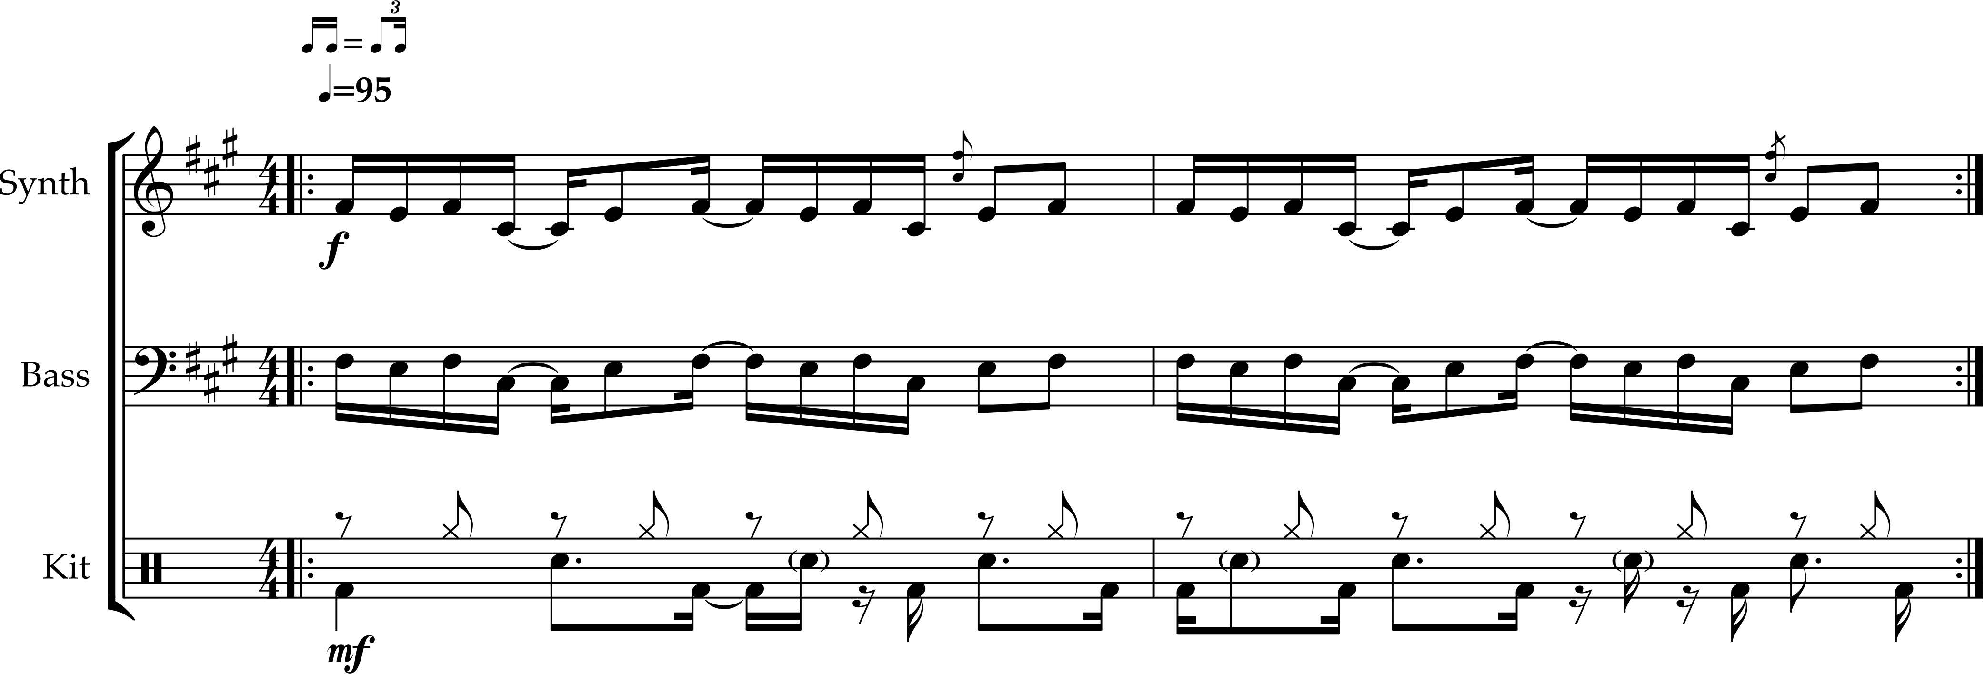
\includegraphics[width=\textwidth]{images/figures/chp 02/000019onebeerintro.pdf}
        \caption{Snapshot of Madlib's first sample in ``One Beer,'' 0:00-0:19.}
        \label{fig:onebeerintro}
    \end{figure}

The first sample sounds like a hook for two reasons. First, it is texturally distinct from the sample 
which underscores the verse portion of ``Huit Octobre,'' the primary instrumental criterion Duinker
identifies for distinguishing hooks from verses.\footnote{\cite{benduinkerSongFormMainstreaming2020}, 99.}
Second, it is created from a shorter, more singularly-focused musical idea. Its harmony, which Adams 
typifies as \emph{repetitive}, is created from two arpeggiations of a one-measure idea in rhythmic unison,
only with slightly varied articulations in each statement.
\footnote{\cite{kyleadamsHarmonicSyntacticMotivic2020}. The three categories Adams provides for 
harmony in hip-hop are repetitive, oscillating, and expansional, all of which I touch on throughout
the course of this chapter.} Overall, this section is sparser in texture and musical material, and 
Madlib uses this contrast as a point of arrival.

Madlib contrasts the first sample with his selection of the second, 0:23-0:25 of the Cortex recording.
Although also pitched up slightly sharper than a whole step, this portion slows to 92 bpm from 95 bpm 
and has a straight rhythmic feel. As Figure~\ref{fig:onebeermain} shows, both the overall musical texture
and harmonic content of this sampled section have thickened in comparison to the first. Playing distinct 
and more typical instrumental roles, the bass and synth underscore a vocal part, and the three create new
oscillating harmonies.

    \begin{figure}[ht]
        \centering
        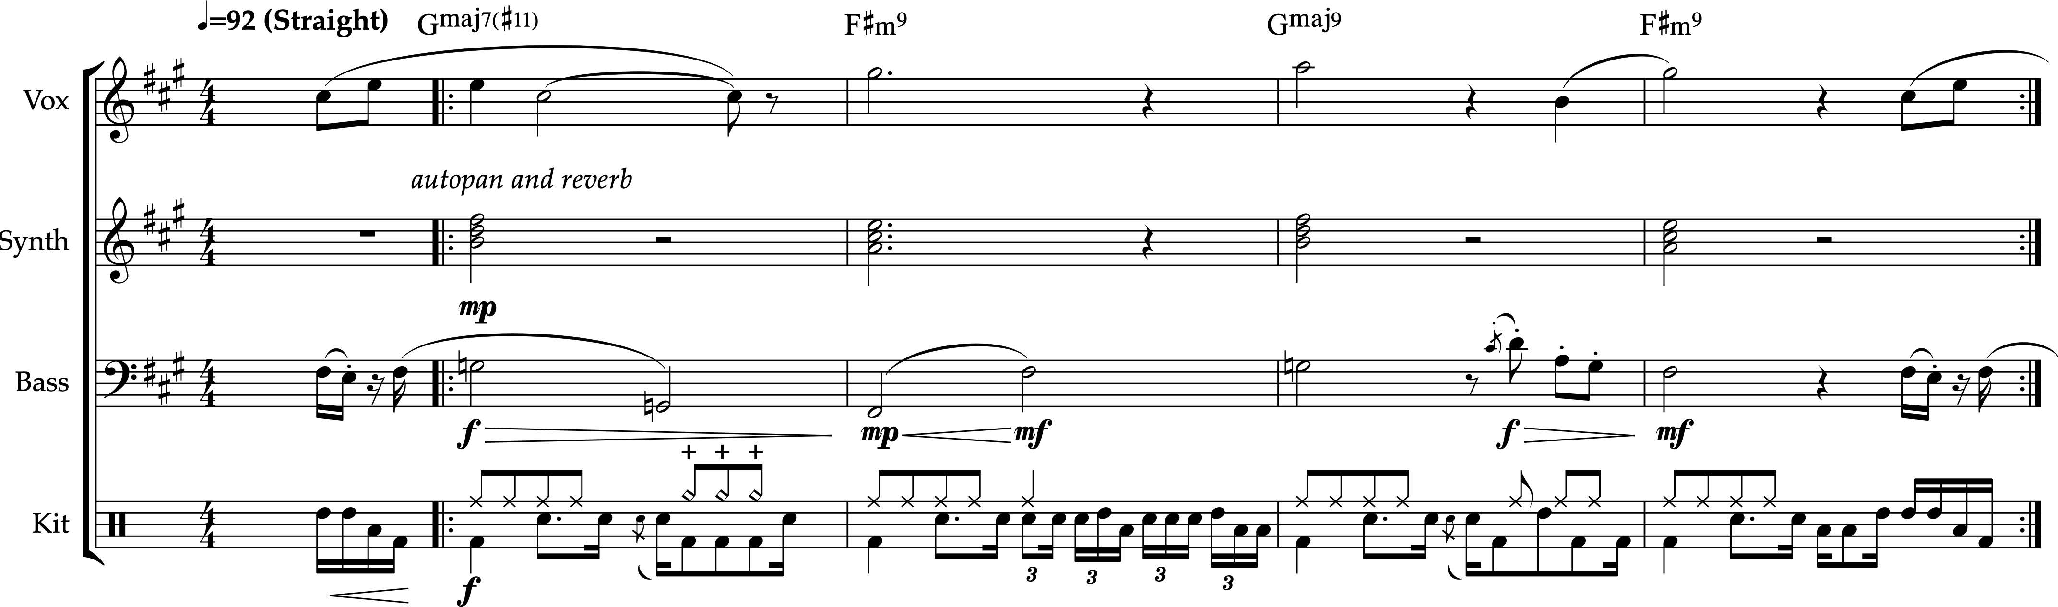
\includegraphics[width=\textwidth]{images/figures/chp 02/020031onebeermain.pdf}
        \caption{Snapshot of Madlib's second sample in ``One Beer,'' 0:20-0:31.}
        \label{fig:onebeermain}
    \end{figure}

Perhaps the most prominent shift in texture comes with the rhythmic complexity of the drum part in the 
second sample. Like the fuller harmony, the drums fill up sonic space using distinctive fills and 
striking timbres throughout the four bar loop; this culminates in the prominence of the two-beat long 
triplet eighth fill in m. 2 of Figure~\ref{fig:onebeermain}. As Schloss notes, producers often choose 
their samples based on the aesthetic delight they experience concerning timbre, especially seeking drum
sounds.\footnote{\cite{josephgschlossMakingBeatsArt2004}, 141-142.} Certainly, this second section 
luxuriates in the sonic quality of the drums.

Comparing the texture, harmony, and groove of each of Madlib's samples illustrates how internally 
varied ``One Beer'' is. Although Madlib makes use of some of the methods of altering samples\textemdash
particularly, choking the sample to delineate sectional transitions\textemdash his primary method of
introducing variety in the main part of ``One Beer'' is through the juxtaposition of the two lead samples.
Juxtaposing musical elements in this manner aligns with Wilson's heterogeneous sound-ideal, particularly
because of the resulting rhythmic clash and  timbral stratification across sample
boundaries.\footnote{\cite{ollywilsonHeterogeneousSoundIdeal1992}, 328-329.}

The final skit section of ``One Beer'' functions as a culmination of Madlib's stylistic juxtapositions. 
The skit's music is built from a looped portion of the soundtrack to ``Dr. Doom, Master of the World,'' 
an episode of the 1981 animated \textit{Spider-Man} television series. He combines dialogue from this 
episode with another selection from ``The Fantastic Four Meet Dr. Doom,'' a 1978 episode of \textit{The 
New Fantastic Four}. Beneath this, Madlib improvises a through-composed drum sequence articulating the
boom-bap structure of kick and snare common in hip-hop. All in one track, Madlib draws on a ``rich 
assortment of multimedia borrowings, references, and parodies that operate in hip-hop music as a
whole.''\footnote{\cite{joannademersSampling1970sHipHop2003}: 42.} This juxtaposition is his method 
of sounding DOOM's particular brand of alternative identity.

\phantomsection
\subsection*{\centering Kendrick Lamar's ``Rigamortus''}
\addcontentsline{toc}{subsection}{Kendrick Lamar's ``Rigamortus''}

    \begin{table}[ht]
        \centering
            \begin{tabular}{|c|c|c|c|l|}
                \hline
                Section  & Timecode & Duration & Sample        & Note \\ \hline
                Intro    & 0:00     & 4 bars   & ``The Thorn'' & \\ \hline
                Hook     & 0:10     & 6 bars   & ``The Thorn'' & Full sample plays \\ \hline
                Verse 1A & 0:27     & 12 bars  & ``The Thorn'' & \\ \hline
                Verse 1B & 0:59     & 10 bars  & ``The Thorn'' & Improvisatory sample choking \\ \hline
                Hook     & 1:26     & 6 bars   & ``The Thorn'' & Lead sample slips backwards \\ \hline
                Verse 2A & 1:43     & 6 bars   & ``The Thorn'' & \\ \hline
                Verse 2B & 2:04     & 8 bars   & ``The Thorn'' & Alternating sample choking \\ \hline
                Hook     & 2:31     & 6 bars   & ``The Thorn'' & Improvisatory sample choking\\ \hline
            \end{tabular}
        \caption{Condensed roadmap to Kendrick Lamar and Willie B's ``Rigamortus.''}
        \label{tab:rigamortus}
    \end{table}

The production team for ``Rigamortus''\textemdash Willie B and Sounwave\textemdash use Willie Jones 
III's up-tempo jazz track ``The Thorn'' as the lead sample,  singling out 0:13-0:20. In ``The Thorn,'' 
the combo groups simple quadruple meter into 3+3+2 beat divisions to underscore a saxophone and 
trombone theme that ends with a pickup figure. This texture is detailed in Figure~\ref{fig:thethornfull},
which highlights the pickup boxed in red.

    \begin{figure}[ht]
        \centering
        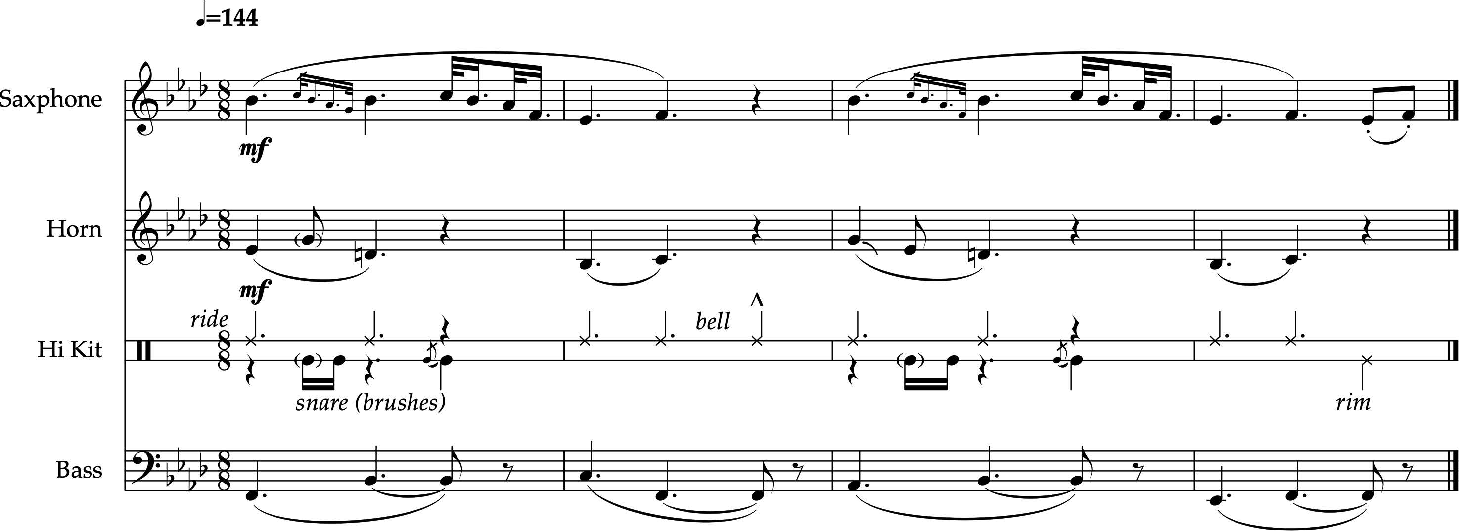
\includegraphics[width=\textwidth]{images/figures/chp 02/013020thethornfull.pdf}
        \caption{Snapshot of the sampled portion of ``The Thorn,'' 0:13-0:20.}
        \label{fig:thethornfull}
    \end{figure}

``Rigamortus'' begins with a nearly unadulterated triggering of the first two measures of the sample.
The only changes the producers make are filtering out the low end and pitching the sample up slightly 
sharper than four semitones. In its new context, the two-bar phrase sounds as a one-bar unit within a 
down tempo hip-hop context. This is confirmed when, as shown in Table~\ref{tab:rigamortus}, the full
four-measure sample is presented beneath Lamar's hook as a two-bar unit. Within the first verse, Willie B
and Sounwave also layer in a drum sequence and sub bass drone on a low A using a filter sweep to demarcate
their entrances. Figure~\ref{fig:rigamortusnoslip} shows the relationship of the sample (now in rhythmic
diminution) to the other elements of the musical texture; this structure repeats unchanged from 0:43-0:55,
with only slight choking of the lead sample.

These new musical elements recontextualize ``The Thorn'' within repetitive harmony that primarily 
sounds an A minor tonic function within a simple quadruple groove. The sample, drum, and bass each 
help ground the listener within Lamar's complex vocal delivery and the complicated approach he uses 
to form with his text. Specifically, Lamar's vocals complicate form with shifts in text and delivery. 
In Verse 2, Lamar briefly recapitulates the ``He Dead!'' call-and-response text from the hook, bisecting
the verse. He also restates the hook text at the beginning of Verse 2A, repeating ``Got me breathin' 
with dragons'' to set up a new rhyme structure and flow in the second verse. At the close of the Verse
2B, Lamar modulates into a higher and more rhythmically intense register, one that he identifies with 
his ``Gemini'' alter-ego.\footnote{\cite{chrismenchTrackingManyVoices2017}.} The producers thus create
contrast through simplicity, using discrete, simplistic musical elements for the track's entirety.

\begin{figure}[ht]
    \centering
    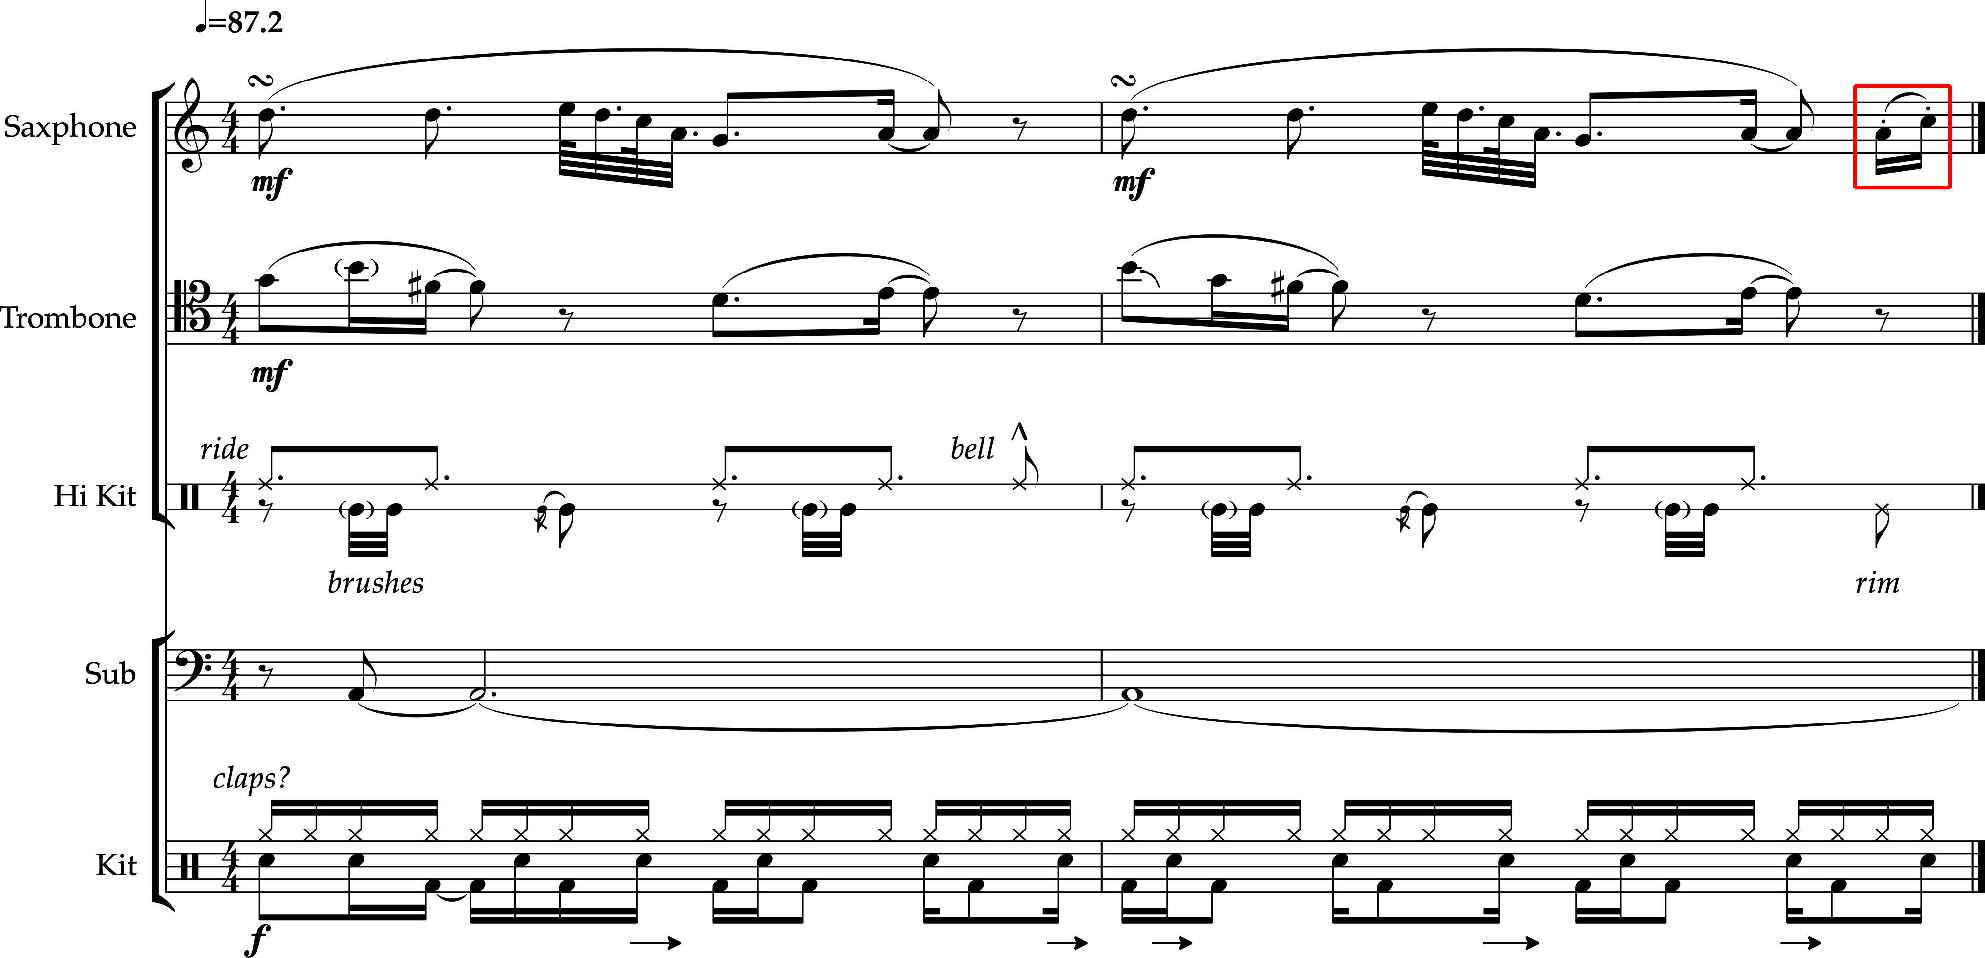
\includegraphics[width=\textwidth]{images/figures/chp 02/043053rigamortusnoslip.pdf}
    \caption{Snapshot of the first verse in ``Rigamortus,'' 0:43-0:55.}
    \label{fig:rigamortusnoslip}
\end{figure}


Although the track's musical components are simplified, Willie B and Sounwave vary their samples and 
loops subtly within the repetitive texture. As Table~\ref{tab:rigamortus} notes, sample choking features
heavily in this track, with the lead sample from ``The Thorn'' rarely playing intact once introduced. 
With Lamar's vocals taking on the ``tendency to fill up sonic space'' of Wilson's heterogeneous
sound-ideal,\footnote{\cite{ollywilsonHeterogeneousSoundIdeal1992}, 328.} the producers opt for 
sample choking as a method of alteration because of its subtractive function, and they employ it 
most drastically when Lamar's vocals reach an apex in Verse 2B. From 2:06-2:18, the lead sample drops
out for measures at a time time, drawing attention to the increasing rhythmic rapidity of Lamar's flow.
Their implementation of sample choking as a tool exists in conversation with Lamar's musical decisions.

\begin{figure}[htp]
    \centering
    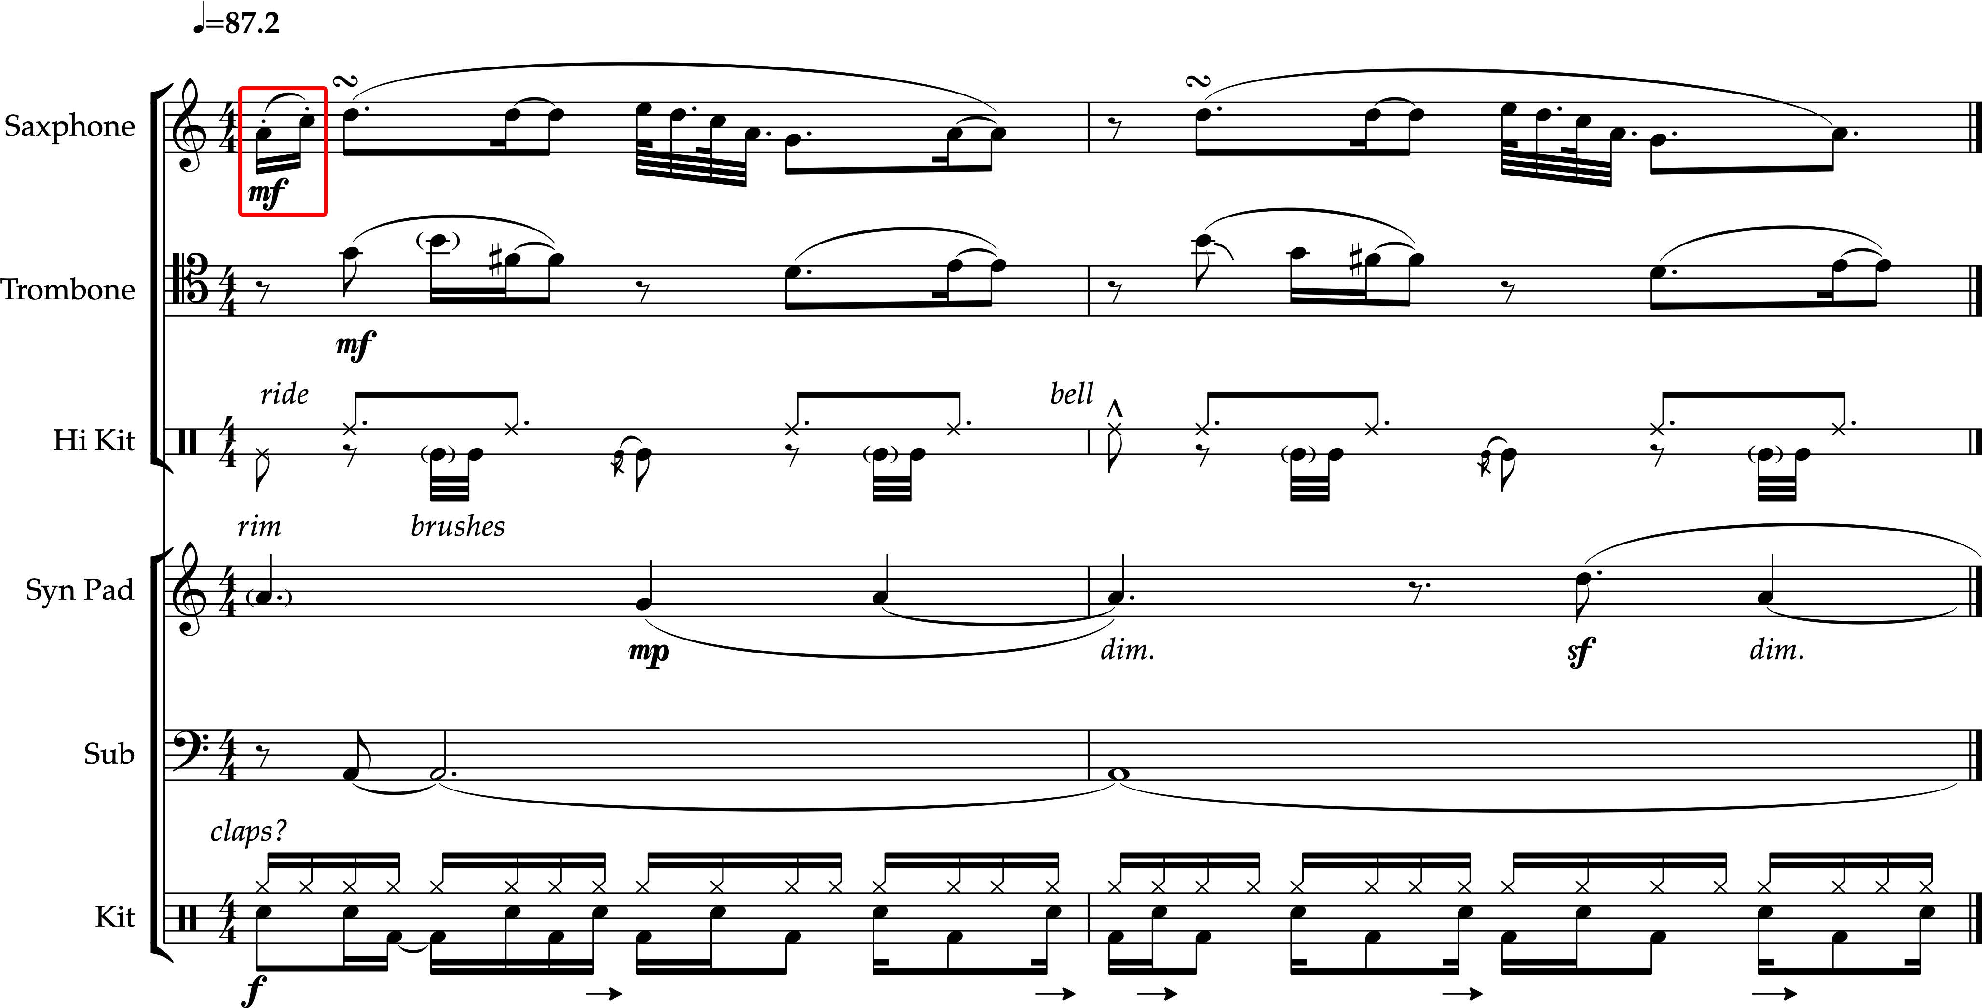
\includegraphics[width=\textwidth]{images/figures/chp 02/126137rigamortusslip.pdf}
    \caption{Snapshot of the first hook in ``Rigamortus,'' 1:26-1:37.}
    \label{fig:rigamortusslip}
\end{figure}

Even more subtly, the producers employ sample slippage as a method of altering the beat in ``Rigamortus.''
Due to the expressive and delayed re-triggering of the lead sample, the microrhythmic relationship 
between musical elements from ``The Thorn'' and the producers' additions exist throughout the work 
in a state of rhythmic flux.\footnote{The phenomenon of sample slippage dovetails with Anne Danielsen's 
work on the Beat Bin and rhythmic tolerance (see \cite{annedanielsenHereThereEverywhere2016}, 
29\textit{ff}. The affective result of these shifts creates a listening experience akin to phasing, 
as samples (albeit sonically discrete ones) move in and out of sync with each other.} Where the pickup
gesture in the saxophone (boxed in red in Figures~\ref{fig:thethornfull}~and~\ref{fig:rigamortusnoslip})
demarcated the end of the lead sample when it was first heard, the sample shifts backwards in the musical
texture throughout the first verse. By the hook, the sample is displaced from its original position in 
the groove, and, as Figure~\ref{fig:rigamortusslip} shows, the pickup figure sounds as a downbeat rather
than a pickup. Both the drum sequence and Lamar's call-and-response vocal articulate this downbeat, which
the saxophone, trombone and sub-bass enter behind by two sixteenth notes. The producers' use of slippage,
then, allows for a sample, which is typically sonically fixed, to become rhythmically fluid.

Willie B and Sounwave's production on ``Rigamortus'' challenges a listener's sense that the lead 
sample on the track is uniformly repetitive. While choking and slipping serve as their primary methods
of altering the sample itself, they also create variety in the beat through the use of digitally-recorded
loops, layering in and out of the mix throughout the track. These loops are all used in conversation 
with Lamar's vocal delivery, helping to create an even greater sense of variety within the musical 
texture. Compared to Madlib's approach to beatmaking, which created variety primarily through the
juxtaposition of disparate samples, Willie B and Sounwave track new elements around the lead sample, 
widening the sample's context. This links the practice of creating variety in sample-based hip-hop 
to another style of production: live-tracked recording.

%\phantomsection 
%\subsection*{\centering Milo and Self Jupiter's ``Ornette's Swan Song''}
%\addcontentsline{toc}{subsection}{Milo and Self Jupiter's ``Ornette's Swan Song}

%\clearpage
\section{Live-Tracked Case Studies}
The second half of this chapter shifts in focus from beats that are sample-based to beats that are
live-tracked. While the distinction between these approaches remains helpful to identifying and describing
the components of a musical texture, it is not a distinction that holds significance beyond this. 
Schloss's ethnographic work in the early-to-mid 2000s Seattle hip-hop scene leads him to the conclusion
that ``the distinction between sample-based and non-sample-based hip-hop is a distinction in
genre.''\footnote{\cite{josephgschlossMakingBeatsArt2004}, 5.} I do not intend to bring in 
such a distinction.

While Schloss's framework may help to explain works in early 2000s underground hip-hop, it becomes
increasingly problematic within modern approaches to music making. When a beat is created in a DAW, 
the distinction between sampling vinyl, using pre-recorded audio or MIDI loops, and live-tracking an
instrument becomes less drastic than within older recording hardware. With the following examples, I aim
to demonstrate that beats are not underground because of the means of generating musical material, but 
rather because of the manipulation of material thereafter.

\phantomsection
\subsection*{\centering Milo's ``Rabblerouse''}
\addcontentsline{toc}{subsection}{Milo's ``Rabblerouse''}

\begin{table}[ht]
    \centering
        \begin{tabular}{|c|c|c|c|l|}
             \hline
            Section & Timecode & Duration & Sample                  & Note \\ \hline
            Intro   & 0:00     & 4 Bars   &                         & Rhodes extends over boundary \\ \hline
            Verse   & 0:08     & 24 Bars  &                         & \\ \hline
                    & 0:14     &          &                         & Drum glitch \\ \hline
                    & 0:36     &          &                         & Drum glitch, bass recomp. \\ \hline
            Outro   & 0:56     & 4 Bars   &                         & Glich, recomp., and choking \\ \hline
                    & 1:03     &          & \textit{Soul Caliber} 2 & \\ \hline
        \end{tabular}
    \caption{Condensed roadmap to Milo and Kenny Segal's ``Rabblerouse''}
    \label{tab:rabblerouse}
\end{table}

Kenny Segal's instrumental for ``Rabblerouse'' creates variety in a complementary fashion to the 
delivery of Milo's text. As shown in Table~\ref{tab:rabblerouse}, ``Rabblerouse'' consists of a single
twenty-four-bar verse framed by two short musical sequences. The track does not end with music; rather, 
it features an unaccompanied vocal sample of the video game character Yoshimitsu from \emph{Soul Caliber 2},
saying ``overconfidence is the greatest enemy'' before giving a battle cry. The sample links ``Rabblerouse''
as an introductory song fragment to Milo's full LP, \emph{So The Flies Don't Come}. It both propels the
listener into the downbeat of the second track, ``Souvenir,'' and links thematically to a line Milo 
delivers in the penultimate track, ``Napping Under the Echo Tree,'' where Milo names himself as the
``Yoshimitsu of Boyle Heights.'' With both sample selection and music, Segal uses ``Rabblerouse'' to 
create instability, urging the listener on toward the album as a whole.

Several structural levels contribute to the fragmentary nature of this opening track. The track is 
structured around an unconventional six-bar chord loop, played in staccato quarter notes on a Fender
Rhodes. Although functional in an E Dorian modal collection, the expansional loop sounds
unresolved.\footnote{\cite{kyleadamsHarmonicSyntacticMotivic2020}. Adams does not make it a 
requisite condition of the expansional harmonic category to function as a complete phrase, although 
he notes that it commonly will.} The C\#$^{sus4}$ harmony that ends the loop, rather than resolving 
the suspension down, cycles back up to an similarly voiced E$^{sus4}$. The stability of this chord 
loop is also challenged by Milo's vocal entrance, which comes after a conventional four bars. The 
Rhodes progression extends over this formal boundary, offsetting the downbeats being projected by 
rapper and producer.

    \begin{figure}[ht]
        \centering
        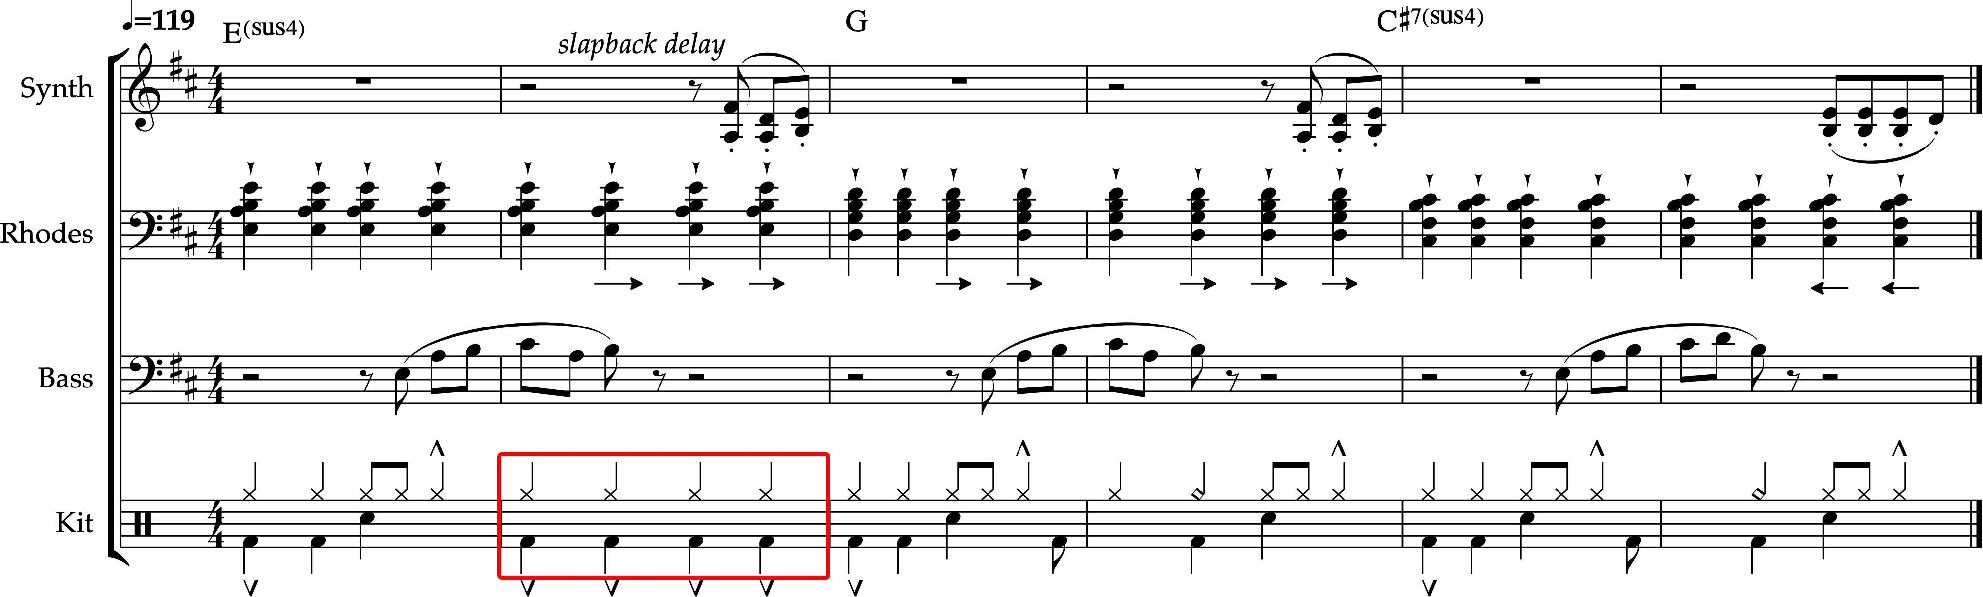
\includegraphics[width=\textwidth]{images/figures/chp 02/012023rabblefirstglitch.pdf}
        \caption{Snapshot of the first drum glitch in ``Rabblerouse,'' 0:12-0:23.}
        \label{fig:rabblefirstglitch}
    \end{figure}

Segal's first notable use of a method of alteration occurs as a response to this dissonance between
the agogic stress of the rapped text and the beat. Boxed in red in Figure~\ref{fig:rabblefirstglitch}, 
Segal uses a glitch in the drum loop to articulate a new point of agogic stress. Measure 2 of the 
figure shows a repetition of four quarter-note kick and hi-hat hits, where Segal has likely selected 
a portion of the drum loop in his DAW and duplicated it four times, restarting the loop in m. 3. This
instance underscores the textual beginning of a new idea: Milo begins ``The wordsmith gets knee-deeper,
beleaguered'' and Segal's glitch transforms the start of the phrase into an upbeat, so that ``deeper''
becomes the strongest metric point of the phrase. Segal's alteration functions as a partial corrective, 
in response to the overall rhythmic complexity introduced in the play between text and music.

    \begin{figure}[ht]
        \centering
        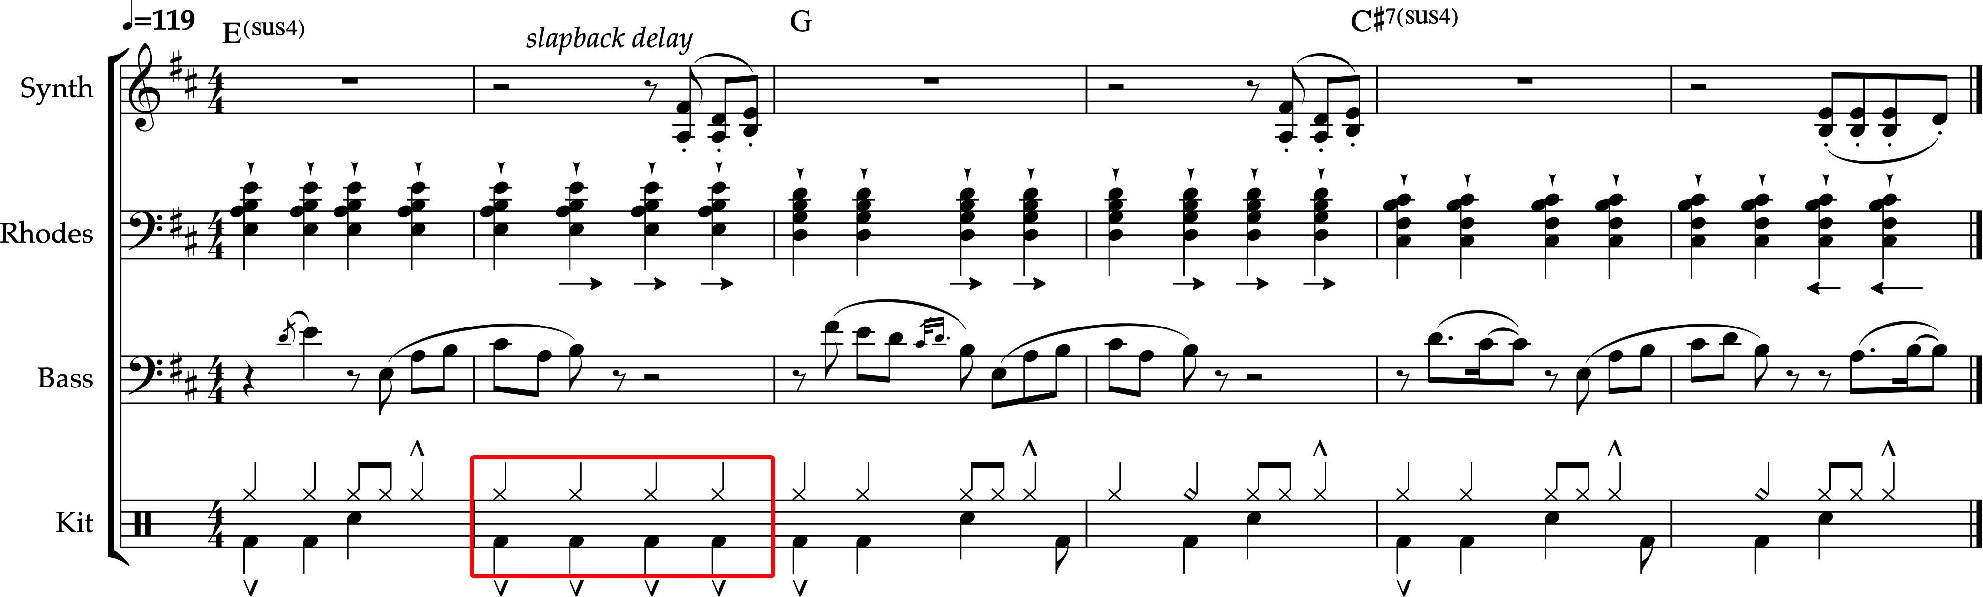
\includegraphics[width=\textwidth]{images/figures/chp 02/036048rabblesecondglitch.pdf}
        \caption{Snapshot of the second drum glitch in ``Rabblerouse,'' 0:36-0:48.}
        \label{fig:rabblesecondglitch}
    \end{figure}

A parallel instance to the first glitch occurs from 0:36-0:48, but its onset is further complicated
by Segal's use of a bass recomposition. Figure~\ref{fig:rabblesecondglitch} shows the loops in this 
moment, with the changes to the bassline implemented by bassist and frequent collaborator of Segal's, 
Mike Parvizi. Parvizi decorates the originally sparse bass lines that begin mid-measure with sleek,
syncopated melodic lead-ins. This busies the texture, while Segal uses another glitch to create agogic 
stress in mm. 2-3. Milo's text \textemdash  ``suits of armor for suicide note authors'' \textemdash again
becomes a point of metric stress, but around this measure, Parvizi's basslines increase the number of
rhythmic onsets within the measure, thereby increasing 
heterogeneity.\footnote{\cite{ollywilsonHeterogeneousSoundIdeal1992}, 328. The ``tendency to create 
rhythmic musical events clash or disagreements of accents'' is the element of the heterogeneous sound 
ideal to which this instance appeals.}

Glitch also functions as the means of suspending rhythmic and metrical clash at the piece's end. As Milo
comes to the end of his verse, Segal uses the same downbeat-repeating drum glitch, pairing it with a 
glitch that extends the E$^{sus4}$ harmony. This point of stasis, though harmonically unresolved, allows
for the listener to hear rhythmic unification for a brief instant, before the texture dissolves and the
Yoshimitsu sample is triggered. Drawing on several methods of altering loops in the beat, Segal brings
together the many fragmentary, disparate pieces of the loop for a brief moment to set a listener up for
what's to come on the record overall.

Segal's fragmentary aesthetic on ``Rabblerouse'' sounds as a mode of alterity because it is uncommon for
a hip-hop beat not to function as a closed loop. The metric dissonance projected from the beginning does
not resolve by the track's end, necessarily drawing a listener in to the text function and pointing 
towards the remaining tracks on the album. This beat is unstable alone, but functions cohesively with 
the sonic palette of Milo's LP \textit{So The Flies Don't Come} as a whole. This technique is predicated 
upon an interest in lyricism and album cohesivity propagated within the underground hip-hop scene.

\phantomsection
\subsection*{\centering billy woods' ``Checkpoints''}
\addcontentsline{toc}{subsection}{billy woods' ``Checkpoints''}

\begin{table}[ht]
    \centering
    \begin{tabular}{|c|c|c|l|}
        \hline
         Section      & Timecode & Duration & Note                          \\ \hline
         Intro        & 0:00     & 8 Bars   & Guitar anacrusis choked       \\ \hline
         Verse 1A     & 0:26     & 22 Bars  & Vocal, synth  anacrusis       \\ \hline
                      & 0:40     &          & Guitar, synth recomp          \\ \hline
         Verse 1B     & 1:06     &          & Synth, drum recomp            \\ \hline
         Interlude 1  & 1:40     & 4 Bars   &                               \\ \hline
         Hook?        & 1:51     & 4 Bars   & All parts anacrusis           \\ \hline
         Interlude 2  & 2:06     & 4 Bars   &                               \\ \hline
         Verse 2      & 2:20     & 15 Bars  & Synth anacrusis glitch        \\ \hline
         
    \end{tabular}
    \caption{Condensed roadmap to billy woods and Kenny Segal's ``Checkpoints.''}
    \label{tab:checkpoints}
\end{table}

Segal also served as the beatmaker for billy woods' ``Checkpoints'' and the \textit{Hiding Places} LP 
from which it comes. Comparing his production techniques across projects for two different emcees shows 
how Segal uses them in response both the artist and the work itself, articulating identity uniquely for 
each. Compared to ``Rabblerouse'' with Milo, Segal's instrumentation on ``Checkpoints'' is at once sparser
and more timbrally intense; the choice to use low register electric guitar with a throatier sound matches 
the more aggressive vocal style woods' employs throughout the track. Similarly to ``Rabblerouse,'' Segal
seems to respond to the text in his articulation of form, working with woods to use techniques that help
create formal contrast. Table~\ref{tab:checkpoints} shows the main formal features: a brief introduction,
followed by two verses of varied lengths, which are divided by an interlude and short vocal section that
could potentially function as the song's hook.

A significant element of the beat is its use of anticipation and anacrusis throughout the 
track.\footnote{I use the term anacrusis as opposed to pickup here because the track does not contain
the final two beats. In the fifteenth bar of the second verse, woods raps through beat two, before 
a static signal sounds for a beat, cutting off before beat four.} Following woods' entrances which 
nearly always come two bars before a downbeat, Segal uses the space beneath that to introduce every 
texture before the downbeat where a loop might be expected to start. Figure~\ref{fig:checkpointsintro} 
shows the entrance of each element from 0:26-0:39 when woods' first verse enters. Accompanying his 
two-beat anacrusis, Segal employs a high synth leadline paired with the guitar loop outlining an F-sharp
power chord. An eighth note before the downbeat, the guitar oscillates to a G harmony, supported by an
anticipation in the kick drum. These anticipations create some rhythmic disorientation in contrast 
to the snare drum, which very clearly articulates backbeats in the section.

    \begin{figure}[ht]
        \centering
        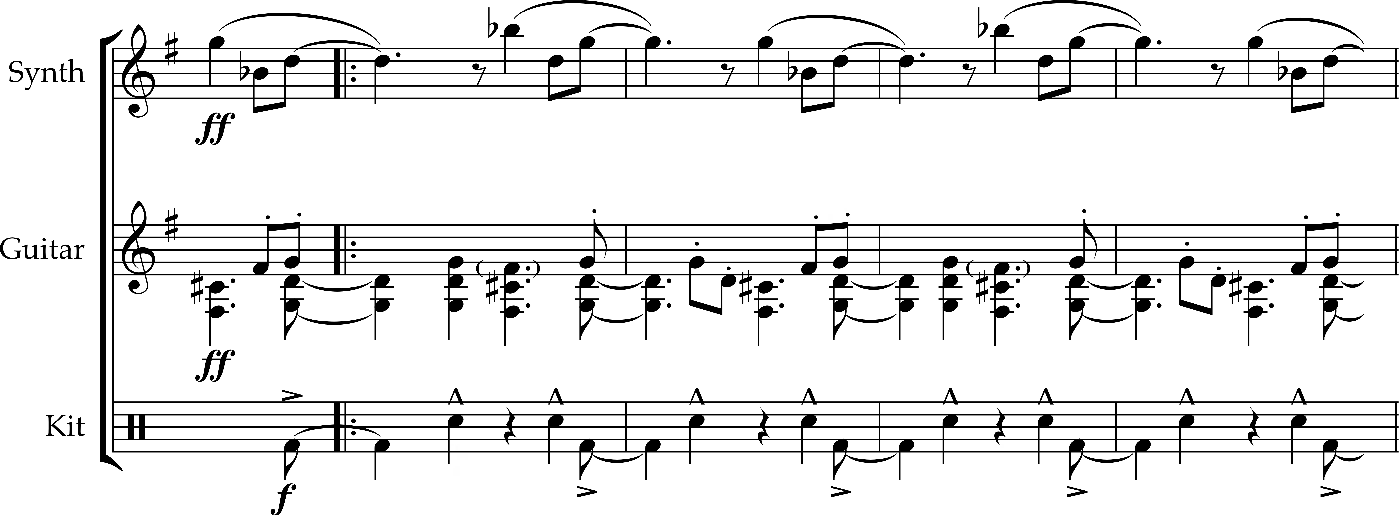
\includegraphics[width=\textwidth]{images/figures/chp 02/026039checkpointsintro.pdf}
        \caption{Snapshot of the beginning of the first verse of ``Checkpoints,'' 0:26-0:39.}
        \label{fig:checkpointsintro}
    \end{figure}


Segal introduces variety into the texture using two significant recompositions of musical material. 
Shown in Figure~\ref{fig:checkpointsmain}, Segal uses a drum recomposition to divide the first verse 
into two eleven-bar units. Following the structure outlined by the kick-snare pattern up to this point,
a crash cymbal emphasizes the downbeat anticipation in the kick, and the same sample sounds a step 
higher along with an open hi-hat sample to emphasize the snare's backbeats. This rock-like groove 
serves as Segal's means of creating variation at an unexpected point of formal division.

    \begin{figure}[ht]
        \centering
        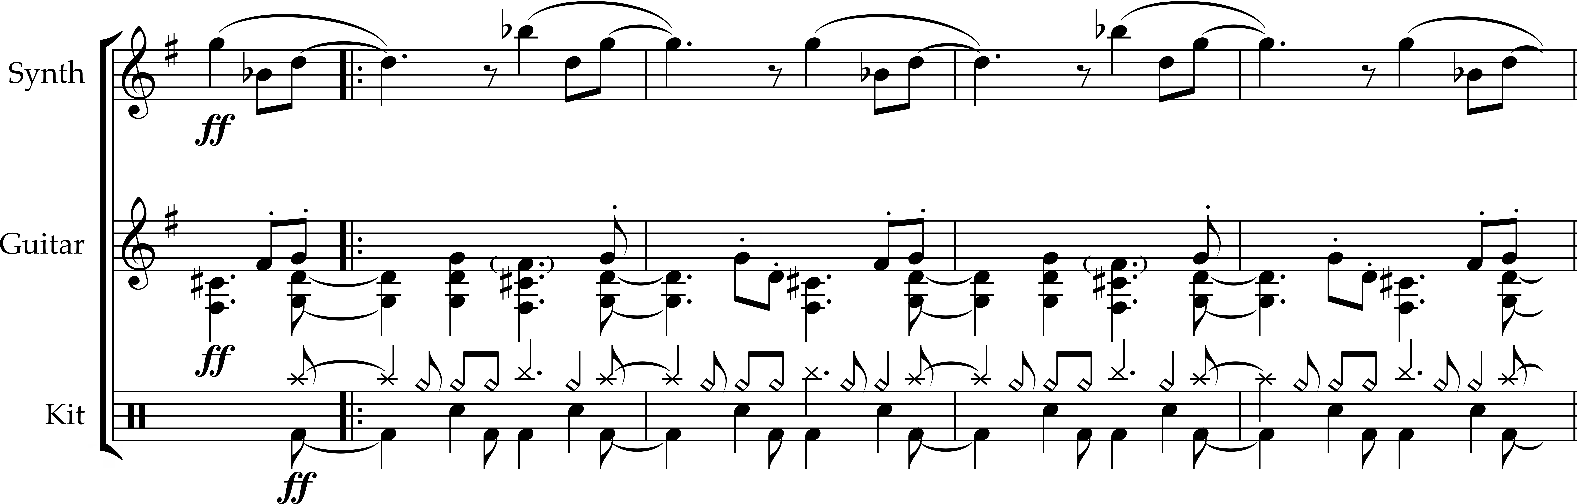
\includegraphics[width=\textwidth]{images/figures/chp 02/106119checkpointsmain.pdf}
        \caption{Snapshot of the drum recomposition in ``Checkpoints,'' 1:06:-1:19.}
        \label{fig:checkpointsmain}
    \end{figure}

Even with woods' vocal delivery signalling a change, the drum recomposition can catch the listener
off-guard. New additions to the drum sequence disrupt the sense of regularity established by the 
kick-snare alternation, especially at a point of division eleven bars into a verse. Moreover, Segal's
choice of drum timbres challenge a listener's sense of genre. Throughout \emph{Hiding Places}, Segal
intentionally uses ``distorted guitars and psych-rock timbres,'' playing with stylistic allusion on 
tracks like ``Checkpoints,'' ``Spongebob,'' and ``Speak Gently.''\footnote{Quoted in 
\cite{backwoodzhiphopKennySegalPresents2019}.} On ``Checkpoints'' specifically, the full drum pattern
engages in allusion while introducing variety.

    \begin{figure}[ht]
        \centering
        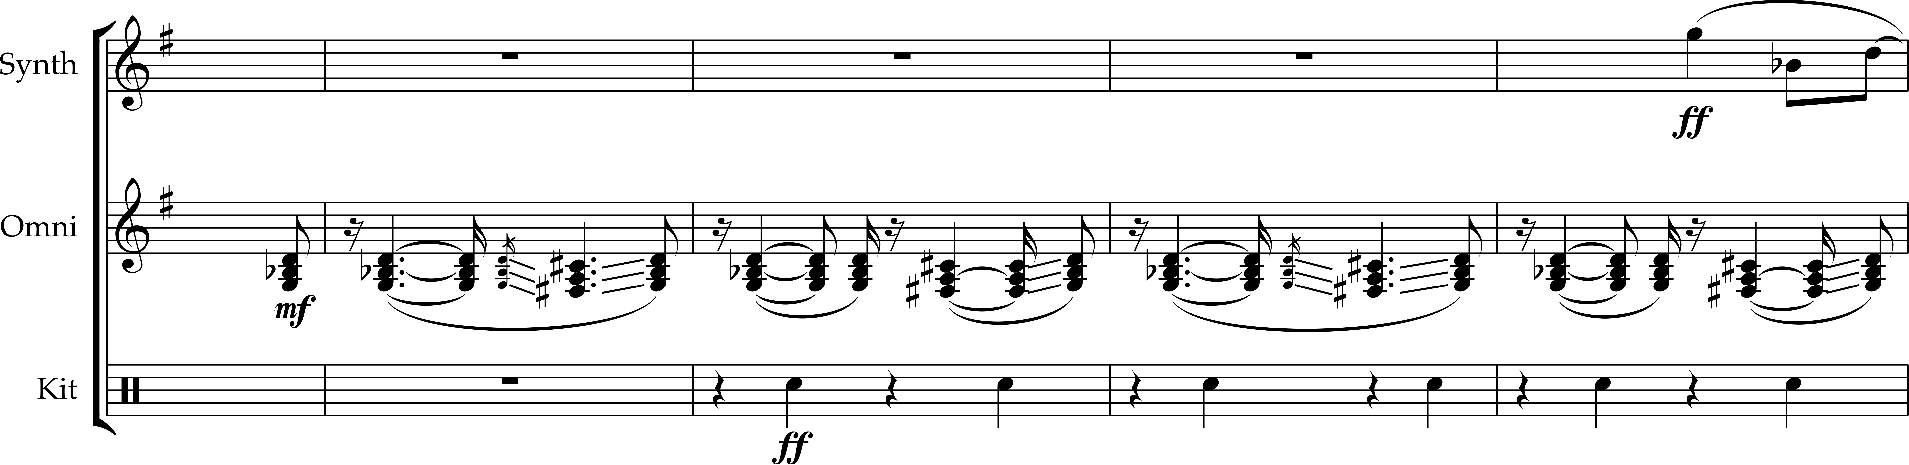
\includegraphics[width=\textwidth]{images/figures/chp 02/040053checkpointsrecomp.pdf}
        \caption{Snapshot of the chordal recomposition in ``Checkpoints,'' 0:40-0:53.}
        \label{fig:checkpointsrecomp}
    \end{figure}

Segal uses recomposition to create formal and textural variety with another significant musical 
element: the chord progression. Figure~\ref{fig:checkpointsrecomp} shows its first entrance, midway 
through Verse 1A. Still in rhythmic anticipation of the downbeat, the chordal loop switches from a 
guitar outlining G and F-sharp power chords to a Suzuki Omnichord planing between G-minor and F-sharp
major triads in the same low-mid layer. Although this recomposition switches instruments, the paired 
range and similar rhythmic placement of the chordal loops aligns the function of these two parts, 
introducing contrasting timbres that take on the same function within the overall 
texture.\footnote{This use of timbral shifts within a shared musical range creates an unblended,
heterogeneous quality within the chordal accompaniment, in keeping with Wilson's heterogeneous 
sound ideal (\textit{cf}.  \cite{ollywilsonHeterogeneousSoundIdeal1992}, 329).}

Each time the chordal recomposition enters, Segal removes all other accompanimental layers
before reintroducing the snare and synth lead. This thinned out texture takes on two distinct 
formal roles. Within the first verse, Segal uses this recomposition to reduce the energy of the 
beat, making the drum recomposition even more drastic when it re-enters with the guitar twenty 
seconds later. This first instance of recomposition allows for a change in energy, creating an 
internal division of the first two verse-parts.

At 1:40, Segal brings the chordal recomposition back to signal a boundary between the verse and 
what follows. For four bars after Verse 1B, the Omnichord and snare sound together, before woods 
re-enters with new text, underscored by the drum kit kit, synth, and guitar also for four bars. 
Segal then switches back to the Omnichord and snare texture for another four bars in anticipation 
of a more fully-orchestrated Verse 2. In these second and third entrances, the recomposition functions
as a formal interlude, affording a weight to the four bars of music and text between them. Indeed, 
woods' text in this section has a certain thematic weight to it; Segal's delineation of form with
recompostion thus helps draw this out.

Segal's use of timbral contrast and sequencing of recompositions within ``Checkpoints'' create
an internal variety within the song form, and plays with the broader, generic context of underground
hip-hop. In Segal's memory of mainstream rap history, the use of rock-like timbres in hip-hop has, 
on occasion, yielded ``disastrously wack results.''\footnote{\cite{backwoodzhiphopKennySegalPresents2019}.}
His choice to navigate this potentially-treacherous sonic territory reveals his willingness to
re-contextualize musical material in play with normative, mainstream expectations. At the same 
time, the use of timbre in ``Checkpoints'' illustrates a desire to do so with specific aesthetic
and compositional ends in mind. Like the sonic profile of his production on \textit{So the Flies 
Don't Come}, this track (and \textit{Hiding Places} as a whole) seem sonically linked to the text, 
themes, and vocal style of the emcee the track exists in service to. Segal's primary concern as a 
producer, then, seems to be sounding an identity \emph{with} the emcee.

%\clearpage
\section{The Co-Creation of Underground Identity}
This chapter positions underground hip-hop producers as coauthors in the creation of a underground
identity with the emcee. Because their work is largely non-textual, underground producers use
normative expectations for form and content in a hip-hop track as a basis for a type of sonic play
that manifests as heterogeneity within a hip-hop beat's construction. Underground producers create
forms that are non-normative, articulating them through sample and loop juxtapositions, and ascribing
formal rhetoric to different portions of the beat through their choice of sequencing. Within 
instrumental sections, producers create heterogeneity with a variety of techniques for manipulating 
sound, four of which I have explored in depth during this chapter. Formal and compositional variety 
functions as a sonic metaphor for the non-normativity of the emcees who rap over these tracks.

\chapter{Structural and Performance Tools for the Underground Emcee}
\onehalfspacing
\section{A Working Definition of Flow}
In comparison to its conceptual counterpart ``the beat'', a ``flow'' resists a clear definition in
academic and technical discourse. While there seems to be some agreement that the beat is comprised
of musically-distinct layers looping throughout a piece, definitions of flow range from anywhere as
specific as ``simply the rhythms and rhymes [a hip-hop song] contains''\footnote{
    \autocite[63]{pauledwardsHowRapArt2009}. While Edwards' statement comes within the context of an
    instruction on rapping (and therefore his reductiveness may be pedagogically useful), this attitude
    toward flow is implied by music academics who transcribe flow primarily on one line of staff notation;
    such transcriptions implicitly show flow as something existing within a fixed (or indiscernible) pitch
    space, with unambiguous, highly discernible rhythms.} 
to as wide-ranging as ``all of the rhythmical and articulative features of an emcee's delivery of 
the lyrics.''\footnote{
    \cite{kyleadamsMetricalTechniquesFlow2009}.} 
Before I name and discuss a few of the stylistic hallmarks of flow in underground hip-hop, it will be
worthwhile for me to construct a definition that ascertains what musical elements comprise it.

Consider, once more, Open Mike Eagle's characterization of his own relationship to MF DOOM's flow:
that Eagle has to be careful with it because of how much time he has spent `in DOOM's mind.'\footnote{
    \cite{estellecaswellRappingDeconstructedBest2016}. For my earlier discussion of this passage and its
    relationship to meditative listening, see Section~\ref{listeningasmeditation}.} 
The fact that Eagle can characterize his relationship to the style of DOOM's flow demonstrates that
flow encompasses more than rhythm and rhyme alone; by themselves these elements do not account for flow
as being tied to an emcee's specific or generic style. Flow, then, should be conceived more broadly than
the manifestation of rhythms through the vocal delivery of rhymes.

At the same time, however, emcees frequently describe flow as text in relation to the music, drawing
contrasts with the non-musically bounded epithet ``poetry.'' The emcee Rakim's oft-cited definition
of rap (that it is ``rhythm and poetry'') creates a distinction between texts that can be rapped and
those that are conceived within the poetic medium. Clarifying this distinction, the emcee Myka 9 of
Freestyle Fellowship offers, ``sometimes I might write a poem, a spoken-word poem, but then morph
that into a rap rhythmically.''\footnote{
    \autocite[63]{pauledwardsHowRapArt2009}.}
Myka 9's insight helps to construct a continuum for rapped text: it exists on a spectrum from
texts that are spoken in musically-bounded ways and non-musically-bounded ways.\footnote{
    Interestingly, rapped verses can be and often are delivered on varying degrees of this
    spectrum. Mitchell Ohriner notes two distinct modes of delivery, which he calls speech-rhythmic
    and music-rhythmic, based on the degree of non-alignment between the musical meter and the 
    degree to which syllable onsets correspond to metrical positions (see 
    \cite{mitchellohrinerLyricRhythmNonalignment2019}.}

This distinction between the construction of the rap as text and its performance as music is
foundational to the method by which I interrogate the concept of flow in this chapter. I believe
the techniques underground emcees employ when rapping can be neatly divided and then analyzed based
on this division, into categories I refer to as \emph{structural} and \emph{performance} techniques.
Structural techniques deal primarily with rap as text, considering its syntactic elements with primacy
over their manifestation as a stream in the musical object. By contrast, performance techniques deal
primarily with rap as music, considering the ways in which an emcee makes manifest the structures
they contrive when composing texts. Moreover, performance techniques encapsulate the decisions made
when treating the voice as an object within a digital recording. With these distinct categories,
I aim to examine how, as Mitchell Ohriner claims, flow ``encompasses phrasing, rhythm, meter, accent,
patterning, and groove, not to mention the relations among these parameters.''\footnote{
    \autocite[28]{mitchellohrinerFlowRhythmicVoice2019}.}

\section{Thesis Statement \& Definitions}
In this chapter, I examine a few notable techniques that underground emcees employ in structuring
and performing their flow, arguing that, like producers, their choice to use these techniques reaches
listeners as underground. The four techniques I define below do not form an exhaustive list, but rather
are salient and illustrative in how they relate to my conception of the subgenre. My terms are also 
divided into the subcategories of structural and performance techniques, a distinction I draw in my 
understanding of how emcees work with the text that makes up their flow. When the underground emcee 
inhabits the role of writer, they experiment with structuring techniques including \emph{pivot rhyme} 
and \emph{closing fragmentation} to craft their verses. Stepping into the recording booth or onto the 
stage, the emcee shifts into their role as rapper and therefore draws on performance techniques such 
as \emph{mimesis} and \emph{processing} to shape their vocal delivery. Each of these techniques serves
as the focus one of the close-readings that follow, so I will clarify their functions before I examine
repertory.

As a device for constructing a verse, a pivot rhyme allows an emcee to execute a shift in end rhyme;
it occurs when the concluding words of the previous bar conjure up an idea that is semantically linked 
to the bar's topic but does not rhyme. In this instance, the rapper chooses to displace the lyric past
the next bar line, allowing that word or phrase to serve as the primary rhyming sound within a new repetition
of the beat pattern. Often the emcee uses this instance as a way to play with audience expectation, taking
the listener's focus on this final rhyme to shift towards a topic semantically distinct from the previous bar.

Underground emcees employ closing fragmentation as another method of structuring a verse, particularly
to mark the end of some sort of formal section. To accomplish this, emcees will deliver a ``full'' textual
phrase, usually structured as a setup and punchline, then signal a close through breaking up and repeating 
the component elements of that textual phrase in a more improvisatory and loosely-organized style of delivery.
Fragmentation and repetition here do not function as they do in the construction of a hook; rather, they
demonstrate to the listener that some larger textual unit\textemdash a phrase, a verse, the song 
itself\textemdash is ending.

With both performance techniques, emcees articulate the role of their voice as a layer \emph{amongst} the rest 
of the mix, rather than the principal element within it. In particular, the use of mimesis, or stylizing vocal 
delivery to mimic other elements in the beat layer, draws attention to the other musical elements in an attempt
to foreground their musicality. This promotes the other musical layer to a co-soloist role, rather than 
functioning as a background loop or layer, allowing the listener to focus on it as more than just accompanimental
structure beneath the vocal flow.

Processing more generally refers to the manipulation of digital audio after its recorded (especially through
the use of EQ, compression, and reverb software or hardware), but here I use it to refer to methods of altering
the vocal signal as a method of electronic composition. In particular, rappers use processing effects like delay, 
distortion, and pitch transposition to alter the audio of their voice during or after tracking it to treat it 
as a musically manipulable element; the vocals here function as \emph{sound} inasmuch as they do text.\footnote{
    My definition of processing here is a broader version of the definition of ``glitch'' in Chapter 2 
    (see p.~\pageref{glitch}.)}
In this way, processing treats the voice as if it were any other musical layer and, as a result, any layer can
be listened with as much consideration as the voice.


%\newpage
\section{Structuring Techniques}
Perhaps more than any other musical element in the rap song, the transcription of flow makes clear the
limitations of staff notation. Throughout this project, my dedication to transcription in standard notation
arises from my desire to mimic what Kofi Agawu conceptualizes as a ``post colonial transcription,'' one based
in an ``ideology of sameness so that\textellipsis we can gain a better view of difference.''\footnote{
    \autocite[67]{kofiagawuInventionAfricanRhythm2003}. Agawu's chapter traces a history of non-African scholars
    transcribing Northern Ewe drumming in a way that both essentializes and exoticizes African music as primarily
    rhythmic and therefore fundamentally different from Western approaches to music making. Although I do not wish
    to employ colonization uncritically as a metaphor for music theory's relationship to hip-hop, I do believe that
    the same essentializing and exoticizing tendencies would manifest if I were to completely avoid standard notation
    for this repertory.}
However, this approach exists at odds with another point Agawu notes: no singular mode of representation can 
sufficiently convey the totality of a musical listening experience.\footnote{
    \autocite[187]{kofiagawuAfricanRhythmNorthern1995}.}
In dealing with flow as an independent, textual structure from its musical manifestation, I will opt to use
another mode of representation: namely, Ohriner's $modulo$ 16 grid transcriptions\footnote{
    For a detailed overview of the system and a few sample transcriptions, see 
    \autocite[xxviii--xl, 7--9]{mitchellohrinerFlowRhythmicVoice2019}.}

Ohriner's method of transcription simplifies certain elements that become problematic when transcribing 
flow in standard notation. First, his 16-point grid for a bar avoids proliferate use of eighth, sixteenth,
and thirty-second notes, not to mention syncopation between them. Subsequently, his method also simplifies 
the naming structure by labeling each metric position with a number from 0--15; one can more succinctly
communicate a syllable landing on ``the third sixteenth note of beat 3'' as position 10, for instance. 
Finally, Ohriner's system does not necessitate a transcriber to choose fixed metrical positions in the 
same way standard notation and adaptations of TUBS for flow do; if a syllable onset occurs slightly before
the beat, this can be accounted for simply by moving the corresponding circle. Although vocal groove and
non-alignment with the meter is not a focus in this chapter, the ability for a system to adapt between
quantized and non-quantized rhythms is foundational to being able to transcribe flow.

\phantomsection
\subsection*{\centering Madvillain's ``Great Day''}
\addcontentsline{toc}{subsection}{Madvillain's ``Great Day''}

Madvillain, the moniker under which DOOM and Madlib released all of their collaborations except for
``One Beer,'' looms large in the world of underground hip-hop. One unrelenting focus of the accolades
their 2004 double LP \textit{Madvillainy} has received is DOOM's flow: in the words of Ta-Nehisi Coates,
``[\textit{Madvillainy}'s] singular sound came mostly from [DOOM's] raspy baritone rendering a sort of
nerdcore poetry.''\footnote{
    \cite{ta-nehisicoatesMaskDoomNonconformist2009}.}

This claim to DOOM's uniqueness, eccentricity, and artistry finds purchase beyond the mythologizing in
which Coates and much of the rest of the hip-hop community partake. Kyle Adams, for instance, notes that
on ``All Caps'' both the melodic samples (various portions of the main theme for the NBC crime drama 
\textit{Ironside}) and DOOM's flow ``[seem] to float free of the meter, being only weakly tethered to
it by the drum sample.''\footnote{
    \cite{kyleadamsMetricalTechniquesFlow2009}. What Adams notes about the \textit{Ironside} sample likely
    bolsters my claim that sample slippage is a frequently employed technique in underground hip-hop production,
    but it is not uniformly employed across Madlib's sampling practice (more on this below).}
Adams arrives at this characterization of DOOM's flow in examining the structure of its syntax: particularly,
how rhymes in ``All Caps'' do not often fall in regular metrical places and that syntactical units (or phrases) 
often cross metrical boundaries. DOOM's novel use of this irregularity, per Adams, contributes to the perception
of DOOM as an alternative rap artist.

While metrical ambiguity and enjambment may play a role in DOOM's sounding as underground on ``All Caps,''
I am hesitant to accept this as the whole picture of DOOM's alternative identity. A counterexample to the
techniques Adams accounts for on ``All Caps'' emerges from the track that immediately follows it on 
\textit{Madvillainy}\textemdash ``Great Day.'' The beat's primary melodic sample comes from ``How Do You
Believe,'' an instrumental funk track by Stevie Wonder, released in 1968 under the alias Evits Rednow.
Madlib aligns the sampled elements (electric piano, harmonica, bass, and auxiliary percussion) closely
with the drum break he uses, ushering in a hypermetric downbeat with a C-sharp minor blues lick every
fourth bar in the A section.\footnote{
    This type of metric regularity also pervades ``One Beer'', where the whole instrumental before
    the skit is sampled from one track by the funk band Cortex (see Section~\ref{samplebased}.)}

Figure~\ref{fig:doomfirstpiv} shows how DOOM, as might be expected, flows with a syntactical structure
of a  similar regularity. Avoiding the downbeat where the sample loops, he raps: ``Mad plays the bass 
like the race card, / Villain on the case to break shards and leave her face scarred.'' Over these two 
bars, DOOM structures a setup and punchline within the confines of the barline, in addition to landing 
the two-syllable rhyme that closes each bar on positions 12 and 14. The internal rhyme in the second bar
(``break shards'') occurs in a metrically weaker position (6 to 8, as opposed to 4 to 6), but falls
within what Ohriner refers to as the same durational segment (in this case, a value of 2 on the grid). 
Rather than interrupt the sense of regularity in the flow, I argue the internal rhyme in this bar 
creates an anticipation for the rhythmically ``restored'' position of the end rhyme.
\clearpage

    \begin{figure}[!ht]
        \centering
        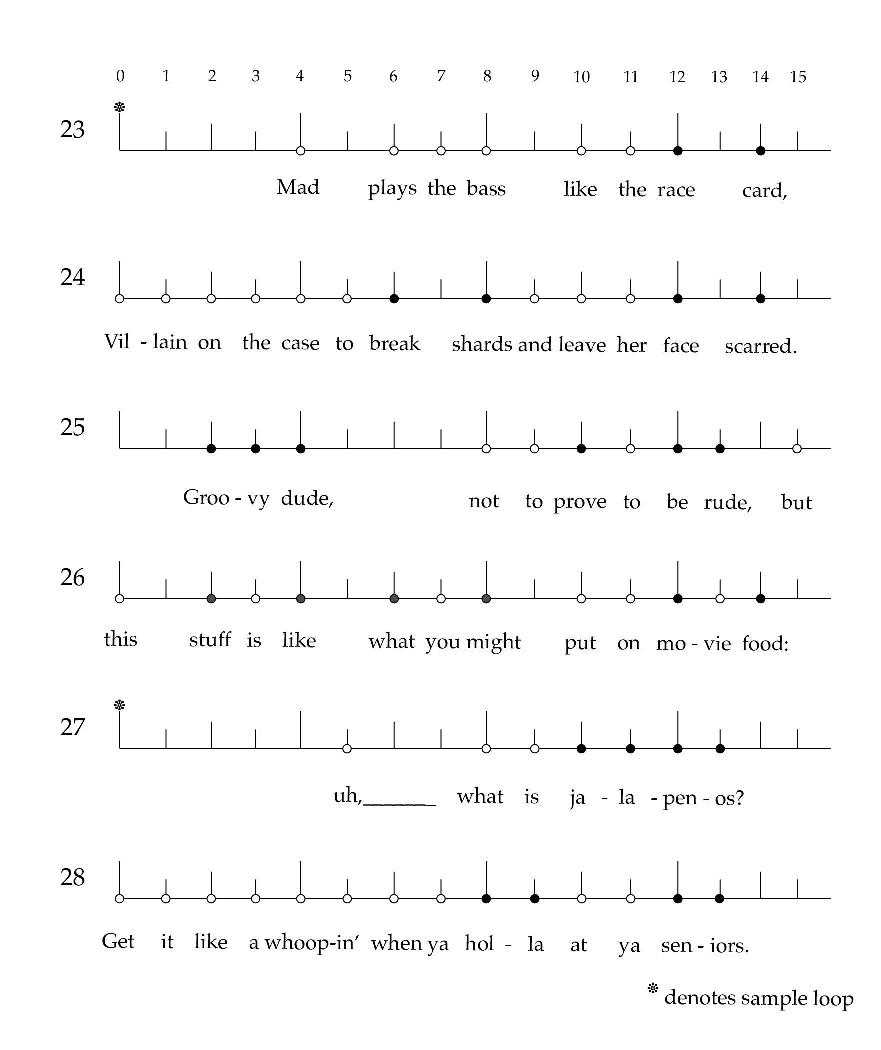
\includegraphics{images/figures/chp 03/059115greatdayfirstpivot.pdf}
        \caption{First pivot in Madvillain's ``Great Day,'' 0:59--1:15.}
        \label{fig:doomfirstpiv}
    \end{figure}

Over the next two bars, DOOM's flow becomes slightly more complex, anticipating the four bar loop
of the sample. Bars 25 and 26 increase the number of syllable onsets from 18 to 22, as well as the 
frequency, position, and syllable count of the rhymes. In the setup bar, DOOM creates an internal 
rhyme with ``Groovy dude'' and ``prove to  be rude,'' each fitting within a durational segment of 2
from positions 2--4 and 10--12, respectively. In the punchline, ``movie food'' once again restores
the metric position of the end rhyme, preceded by two softer, internal rhymes (``stuff is like'' with
``what you might'' falling between 2--4 and 6--8). Despite the increase in internal complexity, the 
syntactic structure of these bars remains normal: DOOM fits a sentence structured ``$x$, but $y$'' 
within the same time span as the previous setup and punchline.

My focus on the regular structure in the first four bars is important for establishing a connection
to the next four, two of which I transcribed as a part of Figure~\ref{fig:doomfirstpiv}. I perceive 
a semantic link in the content of bars 26 and 27 that allows DOOM to pivot to a new rhyme scheme but
in the process invites me as a listener to anticipate something different. My expectation at the end 
of  bar 26 is that DOOM is going to rap about butter: not only because I put it on ``movie food,'' 
but also because he has done so twice already on the album up to this point.\footnote{
    DOOM refers to his ``buttery flow'' on ``Raid'' and Madlib's beats as ``so butter'' on ``All 
    Caps.''}
DOOM, of course, thwarts these expectations, positing ``jalapenos'' as if it were a botched 
\textit{Jeopardy!} answer. He draws out a humorous semantic link between these two bars, drawing
me in to the word which becomes the focus of his rhyme scheme in the oncoming quatrain. With its
final two syllables falling on positions 12 and 13, jalapenos ushers in a set of highly regular
lines, each ending with ``holla at ya seniors,'' ``hashish fienda,'' and ``grass is greener''
in the same metric positions.

DOOM's first humorous pivot and the regularity of the subsequent quatrain provide crucial context
for a similar moment between bars 34 and 35, an instance where I would apply the term pivot rhyme.
Figure~\ref{fig:doomsecondpiv} overviews a quatrain with a similarly regular structure. ``Wishes'' 
falls on positions 11 and 12, displaced 1 position forward from the ends of the two following 
syntactic  closes: ``mad glitches'' and ``jaw twitches.'' The closely related structuring of the 
middle bars of the quatrain set the listener up to hear: ``One thing this party could use is more\textellipsis
booze.''And he makes that ellipsis audible! As a reviewer for \textit{Pitchfork} notes, ``the rhyme's 
pattern and rap's topical stereotype demands the word `bitches,' but [DOOM] hilariously uses `booze'
instead.''\footnote{
    Quoted in \cite{estellecaswellRappingDeconstructedBest2016}.}
Indeed, DOOM's patterning of flow, his regulating of syntactic structure, and his harnessing of
listener's expectations concerning rhyme lead into this moment; he crosses a barline, intentionally,
yet again giving the listener a moment to expect one close to the phrase, before veering off in 
another direction.

    \begin{figure}[!ht]
        \centering
        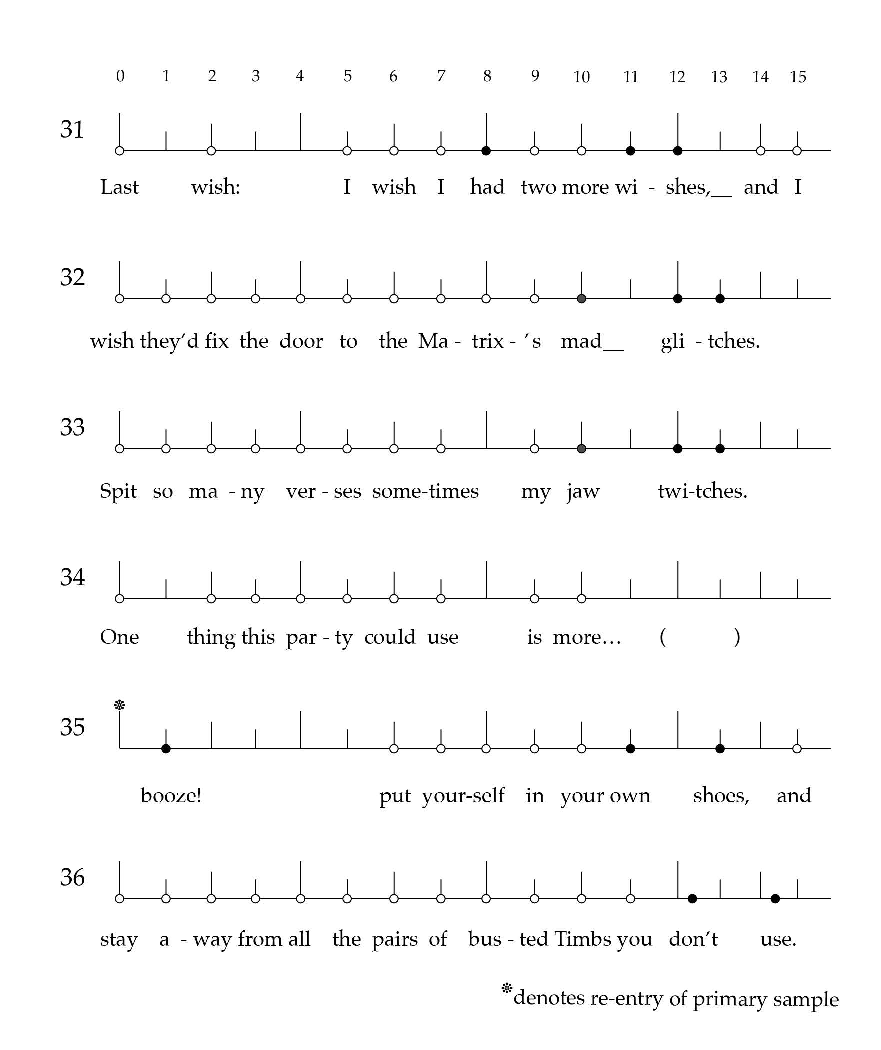
\includegraphics{images/figures/chp 03/121137greatdaysecondpivot.pdf}
        \caption{Second pivot in Madvillain's ``Great Day,'' 1:21--1:37.}
        \label{fig:doomsecondpiv}
    \end{figure}

\phantomsection
\subsection*{\centering Armand Hammer and R.A.P. Ferreira's ``Dead Cars''}
\addcontentsline{toc}{subsection}{Armand Hammer and R.A.P. Ferreira's ``Dead Cars''}

\begin{itemize}
    \item Armand Hammer (billy woods and ELUCID) is a recent premiere (?) underground hip-hop duo out of
    New York, the flagship artist for Backwoodz Studioz
    \item \textit{Shrines} (2019) was a follow up to their critically-acclaimed \textit{Paraffin} (2018) 
    and ``Dead Cars'' a point of exchange with the Ruby Yacht collective; it features R.A.P. Ferreira 
    (owner-operator of the label) and Kenny Segal (a frequent collaborator with both the Ruby Yacht and 
    Backwoodz Studioz roster).
    \item ``Dead Cars'' features a series of short verse-sections from all three artists: at 64 bpm, 
    the three are ``trading 8s''\textemdash  ELUCID begins, woods follows, ELUCID returns, then Ferreira's
    feature enters
    \item Ferreira's verse is marked by a drastic shift in the musical texture: the drums drop out, a
    new Rhodes EP melody is layered in, and reversed audio samples are used to recomposed the chord
    loop
    \item The transcription Figure~\ref{fig:roryclosingfrag} picks up in the early mid-verse, 
    two bars prior to the drum's re-entry
        \begin{itemize}
            \item Ferreira's verse, although slightly varied in the placement of syllables throughout,
            remains consistent in it's placement of rhyming syllables slightly in anticipation of positions
            4 and 12; in lieu of snare drum hits, these orient us within the instrumental texture
            \item As the drums re-enter, Ferreira delivers only two syntactic units (``Bronze Kafka
            metamorph, Black Orpheus set the course / in the Backwoodz, jiggin' with no remorse'') throughout
            the second half of his verse part.
            \item This technique functions as a kind of signposting; we know once Ferreira begins
            fragmenting and repeating text that the verse (or verse-part, in this case) is drawing
            to a close. I call this \textit{closing fragmentation}
        \end{itemize}
    \item This technique resembles the two of Duinker's definitions: hook-sections are typified by
    lyrical repetition and fragmentation, and looser-organized vocal sections comprised of ``ad-hoc,
    ametric vocals, skits, or\textellipsis [rapping] that doesn't function like a verse or hook.''
        \begin{itemize}
            \item Duinker's categorizations make some helpful distinctions, but Ferreira's closing
            fragmentation technique avoids a clear fit in one section or the other. 
            \item The lyrics are fragmented/repeated, but Ferreira situates them within the verse's
            rhyme scheme and patterning of the vocals.
            \item Their content be characterized as the type of ``hype'' vocals Duinker identifies
            (Ferreira is doing is due dilligence by shouting out Backwoodz as a collective, much
            like a hype vocalist shouts out producers involved with the making of a track), but
            the vocals are still presented as if they are a verse-part, not something appended to
            the end of a track.
            \item Closing fragmentation, then, becomes a valuable way to describe an emcee's use
            of fragementation and repetition within the context of verse, if the emcee uses those
            tools to create a ``tag'' like ending.
        \end{itemize}
    \item As a listener, I've encountered closing fragmentation most prominently in Ferreira's 
    discography, but the tool is not idiosyncratic to his approach. On ``Dead Cars,'' both ELUCID
    woods employ it to a lesser extent at the close of their verse-parts. Additionally, other members
    of the Ruby Yacht collective, especially Pink Navel and S.AL, have picked up on the technique.
\end{itemize}

    \begin{figure}[!htp]
        \centering
        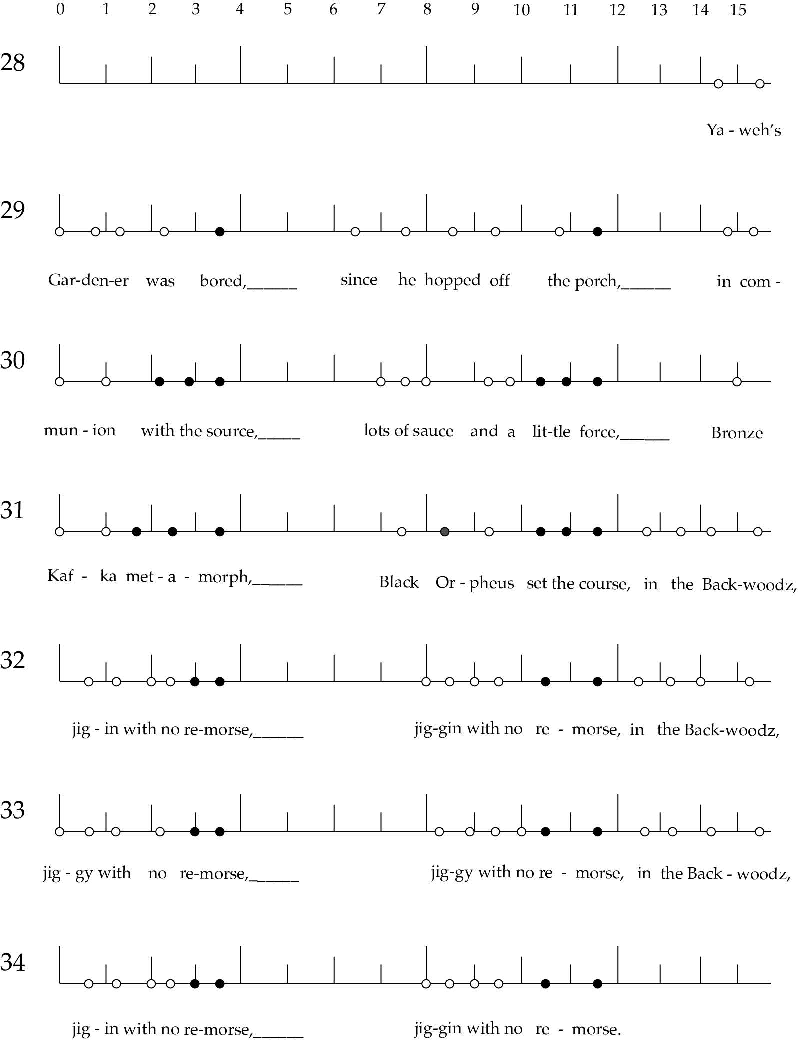
\includegraphics{images/figures/chp 03/144206deadcarsendfrag.pdf}
        .\caption{R.A.P. Ferreira's closing fragmentation in ``Dead Cars,'' 1:44--2:06.}
        \label{fig:roryclosingfrag}
    \end{figure}


\newpage
\section{Performance Techniques}
\phantomsection
\subsection*{\centering R.A.P. Ferreira -- ``NONCIPHER''}
\addcontentsline{toc}{subsection}{R.A.P. Ferreira's ``NONCIPHER''}
    
    \begin{figure}[!htp]
        \centering
        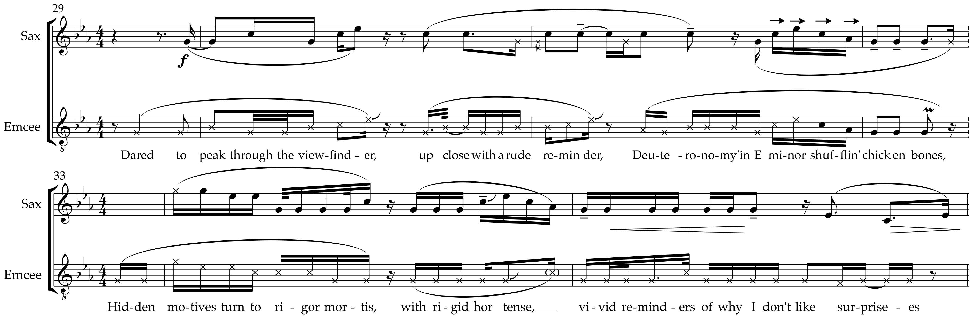
\includegraphics{images/figures/chp 03/120137nonciphermimesis.pdf}
        \caption{Mimesis in R.A.P. Ferreira's ``NONCIPHER,'' 1:20--1:37.}
        \label{fig:rorymimesis}
    \end{figure}
    \begin{itemize}
        \item Transcription of ``framing region'' and Verse 2, Vocal and Sax Lines
        \item Rory draws the ear to the saxophone work, live-tracked by Aaron shaw
        \item Demonstrating his own musical ear; showing that flow has a melodic dimension
    \end{itemize}
  
\phantomsection
\subsection*{\centering Moor Mother and billy woods (ft. Elucid)  -- ``Tiberius''}
\addcontentsline{toc}{subsection}{Moor Mother, billy woods, and Elucid's ``Tiberius''}

\begin{figure}[!p]
    \centering
    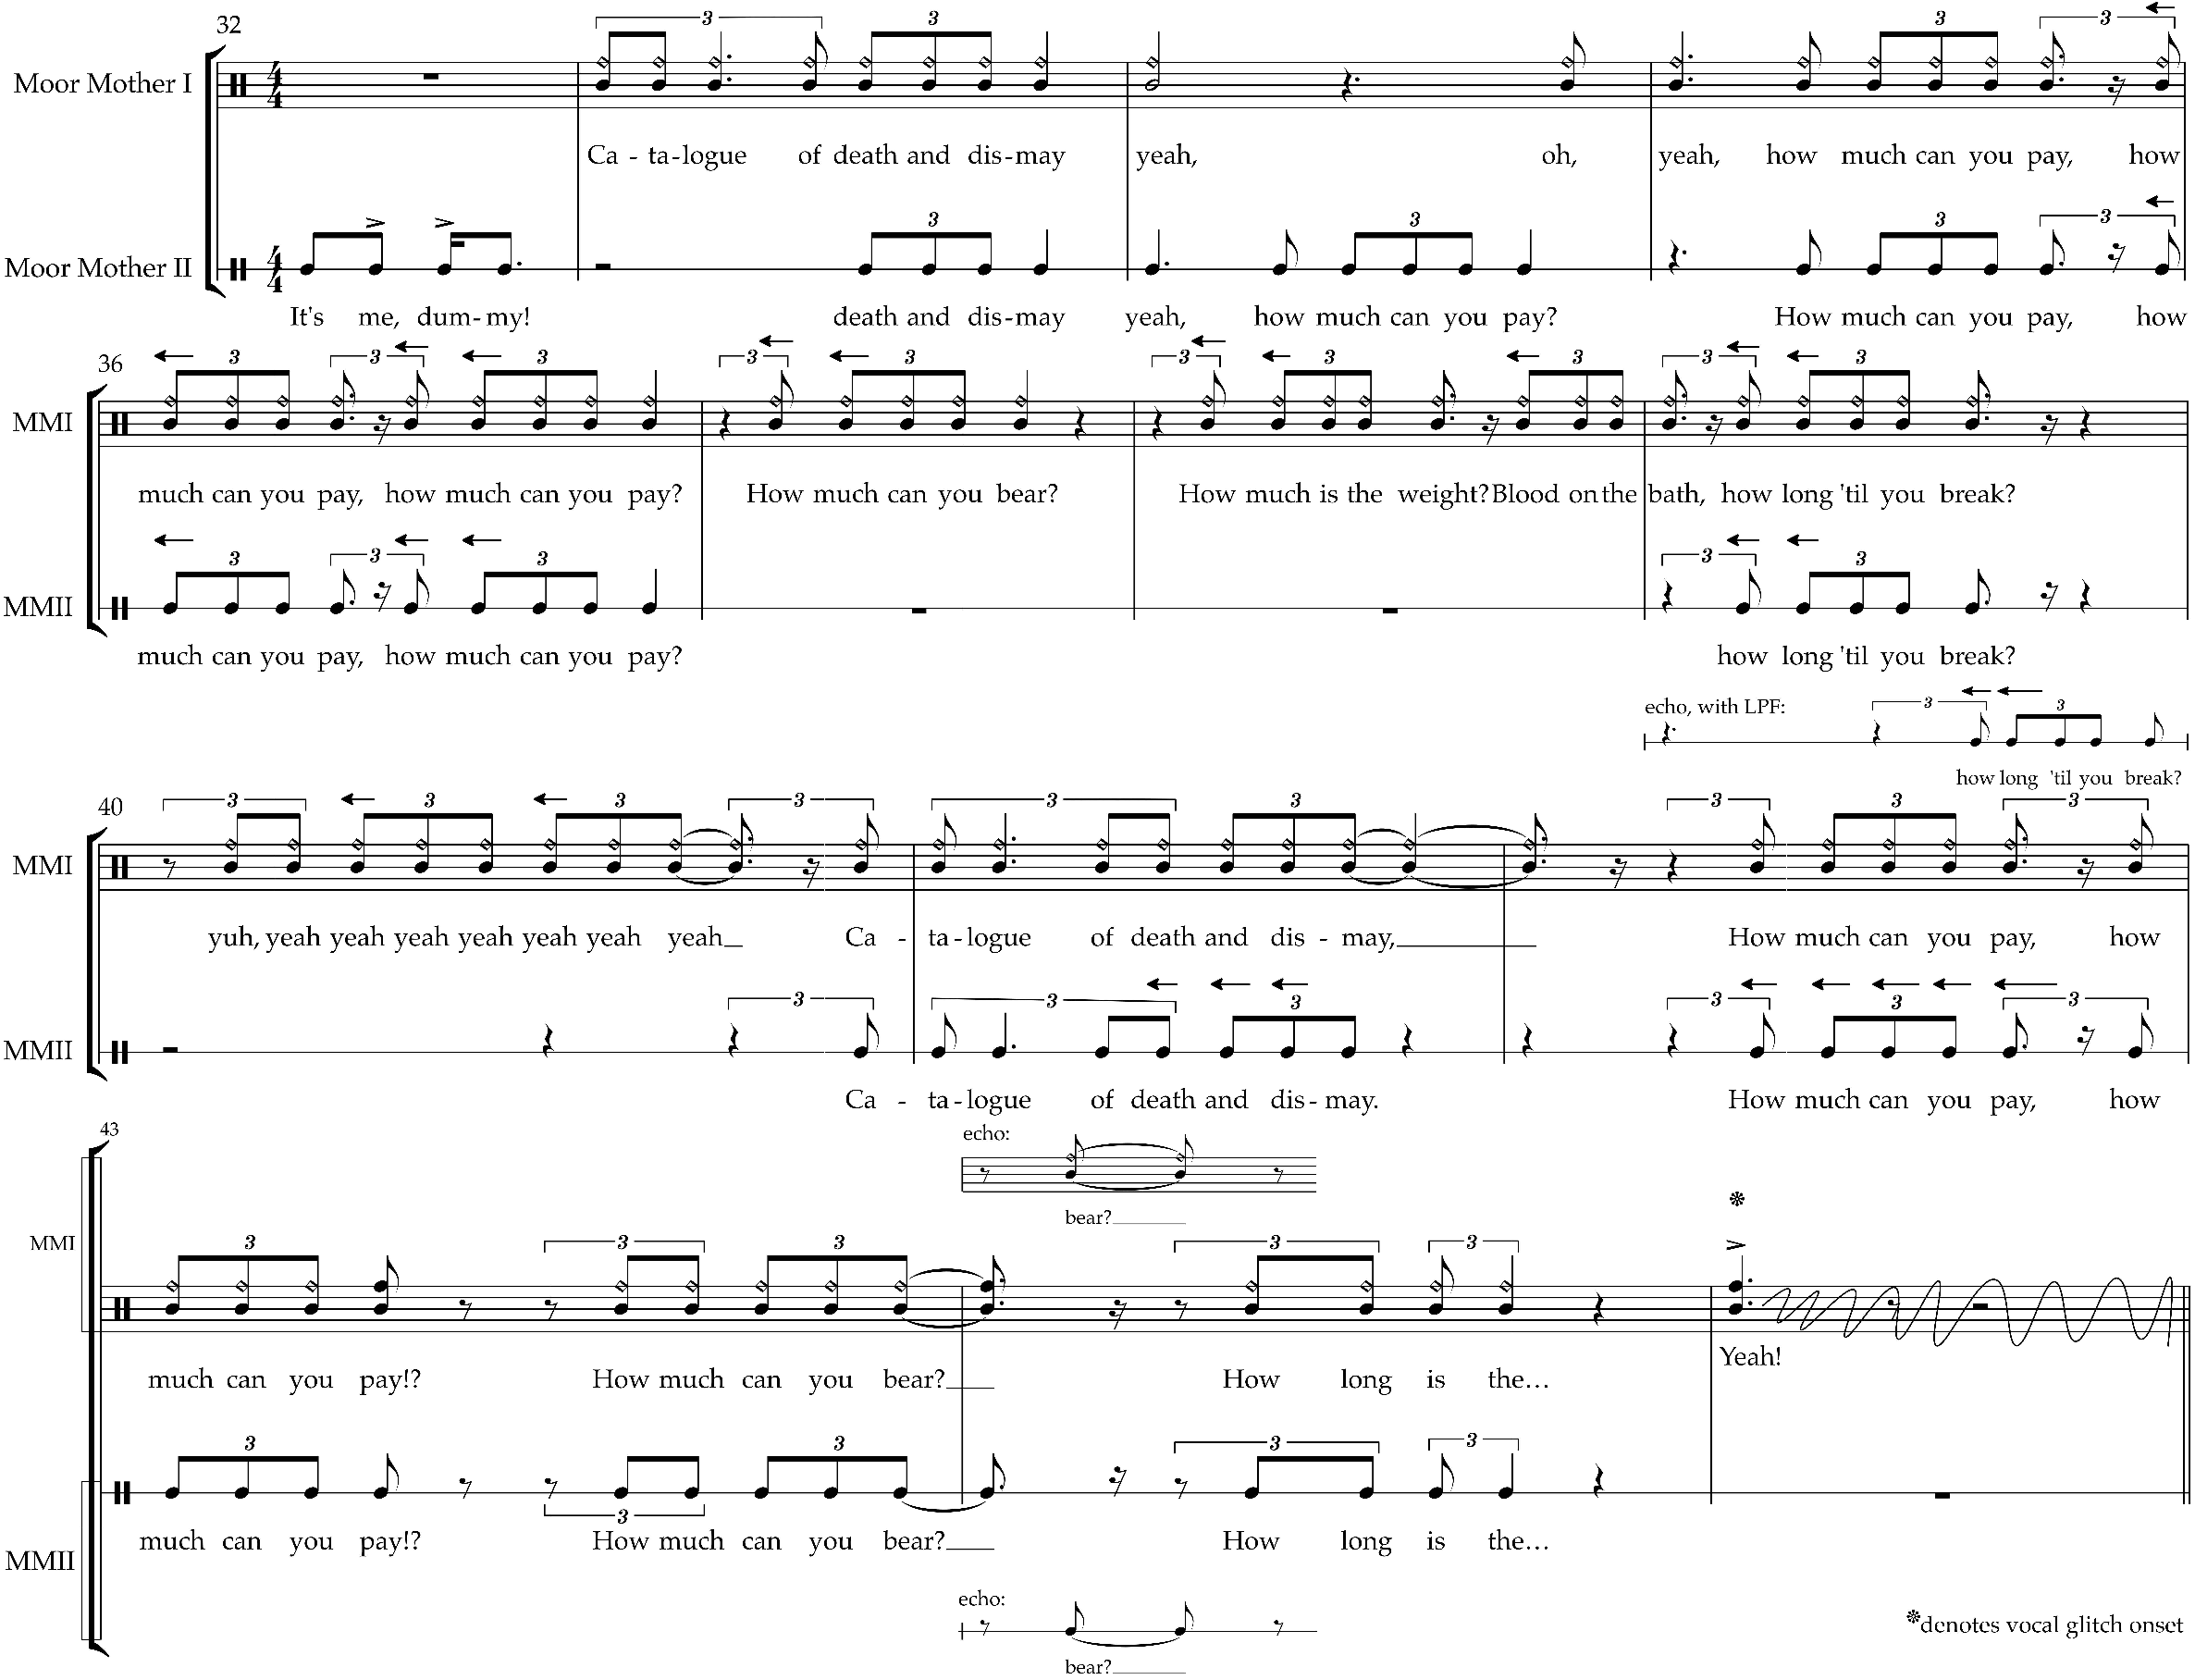
\includegraphics[width=\textwidth]{images/figures/chp 03/107136tiberiusprocessing.pdf}
    \caption{Vocal processing in Moor Mother and billy woods' ``Tiberius,'' 1:07--1:37.}
    \label{fig:moormotherprocess}
\end{figure}

%---------------------------%

\singlespacing
\printbibliography
\addcontentsline{toc}{chapter}{Bibliography}
\nocite{*}

%---------------------------%
\chapter*{Appendix}
\addcontentsline{toc}{chapter}{Appendix}
\onehalfspacing
\appendix \label{appendix:fullroadmaps}
\renewcommand{\thetable}{A.\arabic{table}}
\setcounter{table}{0}

The following tables are full versions of the ``roadmap'' style of transcription employed in
Chapter 2 (beginning on p.~\ref{chapter2}). While the in-chapter tables spotlight distinctive 
textural moments in each instrumental, they do no not separate out the musical textures and 
detail their interaction, in order to save space. In these expanded versions, I give each 
textural layer its own column, and I notate entrances using either the sample source's name 
for the layer or some short descriptive word, phrase, or musical indication to communicate 
its function to a listener. Where appropriate, I give chord names to chart harmonic progressions. 
When a sample or loop repeats within a given timecode designation, I use a notation to mimic 
repeat signs from staff notation and give a multiplier if there is more than one repetition 
(||: $x$ :|| x3, x4, etc.). When higher order repetitions occur across timecode designation, 
I borrow another facsimile of a repeat sign from musical notation, again specifying the 
number of times a full unit is repeated with a multiplier when necessary (•//• x3, x4, etc.).

Rather than using bars and beats to indicate lengths of time in the music, these expanded 
roadmaps opt for a more production-forward way of keeping track of time: inclusive timecode 
designations. Indeed, I give the full timecodes so that a reader can clearly see how long a 
sample or loop lasts, in addition to noting the ways the texture changes via layering and 
the other methods of alteration producers use. This method of time-keeping also allows for 
a more user-friendly experience when listening through a piece while reading these transcriptions. 
Ideally, a listener can jump to a timecode of their choosing, and listen through to hear 
individual layers, and see the corresponding text signaled in the column designated for the 
rapper. Instead of having to count beat units and groups of bars to keep track of time, the 
layout condenses how a producer might see the musical elements in a digital audio workstation: 
as individual blocks of sound built from loops and samples, coming in and out of a the 
musical texture.


\begin{sidewaystable}[t]
    \small
    \centering
\begin{tabular}{|c|c|c|c|c|c|}
     \hline
     Timecode  & DOOM & Lead Sample & Bass & Drums & Vocal Sample \\ \hline
     0:00-0:14 & ``I get no kick\textellipsis'' & ||: ``Huit'' I :|| x4 & ||: ``Huit'' I :|| x4 & ||: ``Huit'' I :|| x4 &  \\ \hline
     0:15-0:17 & ``I get a kick outta\textellipsis'' & •//• x1 & •//• x1 & •//• x1 & \\ \hline
     0:18-0:19 & ``brew!'' & & & & \\ \hline
     0:20-0:40 & ``There's only one beer\textellipsis'' & ||: ``Huit'' II :|| & ||: ``Huit'' II :|| & ||: ``Huit'' II :|| &  \\ \hline
     0:41-1:01 & ``Told him tell 'em\textellipsis'' & •//• x2 & •//• x2 & •//• x2 & \\ \hline
     1:02-1:21 & ``He went to go laugh\textellipsis'' & •//• x2 & •//• x2 & •//• x2 & \\ \hline
     1:22-1:42 & ``(skeezer) eye, and squeeze\textellipsis'' & •//• x2 & •//• x2 & •//• x2 & \\ \hline
     1:43-1:57 & ``Looser than a pair\textellipsis'' & ||: ``Huit'' I :|| x4 & ||: ``Huit'' I :|| x4 & ||: ``Huit'' I :|| x4 & \\ \hline
     1:58-1:59 & ``Few could do it\textellipsis'' & •//• x1 & •//• x1 & •//• x1 & \\ \hline
     2:00-2:02 & ``Take it from the dude\textellipsis'' & •//• x1* & •//• x1* & •//• x1* & \\ \hline
     2:03-2:23 & ``He plot shows like...\textellipsis'' & ||: ``Huit'' II :|| & ||: ``Huit'' II :|| & ||: ``Huit'' II :|| & \\ \hline
     2:24-2:44 & & •//• x2 & •//• x2 & •//• x2 & \\ \hline
     2:45-3:05 & & •//• x2 & •//• x2 & •//• x2 & \textit{Spider-man} I \\ \hline
     3:06-3:50 & & ||: \textit{Spider-Man} :|| x8 & SP-303 & SP-303 & \textit{Spider-man} II \\ \hline
     3:51-3:55 & & •//• x1* & •//• x1* & •//• x1* & ``Your attempts\textellipsis'' \\ \hline
     3:56-4:18 & & •//• x4  & •//• x4 & •//• x4 & \textit{Spider-man} III \\ \hline
\end{tabular}

\vspace{0.2cm}
\hspace{5.5in}{*choked on last two beats}
    \caption{Full roadmap to MF DOOM and Madlib's ``One Beer''}
    \label{tab:onebeerfull}
\end{sidewaystable}
\clearpage
\singlespacing

\begin{sidewaystable}
    \centering
    \begin{tabular}{|c|c|c|c|c|c|c|}
     \hline
      Timecode  & Kendrick & Lead Sample & Drums & Bass & Synth & SFX \\ \hline
      0:00-0:10 & ``Alright\textellipsis''* & ||: ``Thorn'' :|| x4 & & & & \\ \hline
      0:11-0:15 & ``Got me\textellipsis''* & •//• x2  & & & & \\ \hline
      0:16-0:26 & ``(bas)tard, I'm Marilyn\textellipsis'' & ||: ``Thorn'' II :|| & & & & \\ \hline
      0:27-0:32 & ``this is rigor mortis\textellipsis'' & •//• x1 & & & & Filter Sweep** \\ \hline
      0:33-0:42 & ``orbit, you an orphan\textellipsis'' & •//• x2 & ||: 2-bar† :|| & & & \\ \hline
      0:43-0:53 & ``(for)gin' all my signatures\textellipsis'' & •//• x2† & ||: 2-bar :|| & Drone & & \\ \hline
      0:53-0:58 & ``(suit and) tie  are suitable\textellipsis'' & •//• x1† & •//• x1 & & & ``Hey!''s \\ \hline
      0:59-1:04 & ``(He) dead! Amen! That's what\textellipsis'' & •//• x1† & •//• x1 & & & •//• \\ \hline
      1:05-1:15 & ``(Ferra)gami, so many\textellipsis'' & •//• x2† & •//• x2 & •//• & & \\ \hline
      1:16-1:25 & ``(Wrest)ling? That's irrelevant\textellipsis'' & •//• x2† & •//• x2 & & & •//•* \\ \hline
      1:26-1:30 & ``(He) dead! Yup yup! Amen!\textellipsis'' & •//• x1† & •//• x1 & •//• & G-A, D-A & \\ \hline
      1:31-1:41 & ``Got me breathin'\textellipsis'' & •//• x2† & •//• x2 & •//• & •//• & Delay Throw** \\ \hline
      1:43-1:47 & ``Got me breathin'\textellipsis'' & •//• x1† & 2-bar & & & \\ \hline
      1:48-1:57 & ``I rapped 'em and made 'em\textellipsis'' & •//• x2† & •//• x2 & •//• & & \\ \hline
      1:58-2:08 & ``my casualty, and it's casually\textellipsis'' & •//• x2† & •//• x2 & & & ``Hey!'' + Dly** \\ \hline
      2:09-2:19 & ``And I go visit\textellipsis'' & •//• x2† & fill** & Subs & & ``Hey!''s \\ \hline
      2:20-2:30 & ``(men)tion, how the far\textellipsis'' & •//• x2† & ||: 2-bar :|| & & •//• & •//• \\ \hline
      2:31-2:35 & ``(He) dead! Yup yup! Amen!\textellipsis'' &  •//• x1† & •//• x1 & & & \\ \hline
      2:36-2:41 & ``Got me breathin'\textellipsis'' & •//• x1† & •//•x1 & & & \\ \hline
      2:42-2:47 & ``(He) dead! Yup yup! Amen!\textellipsis'' & •//• x1† & •//•x1† & & & \\ \hline
\end{tabular}

\vspace{0.2cm}
\hfill{*enters at the 2nd sample repetition}

\hfill{**enters on the last two beats}

\hfill{†sample is choked, shifted, or otherwise altered}
    \caption{Full roadmap to Kendrick Lamar, Willie B, and Sounwave's ``Rigamortis''}
    \label{tab:rigamortusfull}
\end{sidewaystable}

\begin{sidewaystable}[t]
    \centering
    \small
    \begin{tabular}{|c|c|c|c|c|c|c|c|} 
        \hline
         Timecode & Milo & Drums & Rhodes & Bass I & Synth & Bass II & Vocal Sample \\ \hline
         0:00-0:11 & ``They couldn't\textellipsis''* & 6-bar halftime & 3-chord loop & & & & \\ \hline
         0:12-0:23 & ``(merci)ful, I'm\textellipsis'' & •//• & •//• & ||: E-B :|| x3 & fourths & & \\ \hline
         0:24-0:35 & ``I might\textellipsis'' & •//• & •//• & •//• & •//• & & \\ \hline
         0:36-0:47 & ``evening, I\textellipsis'' & •//• & •//• & •//• & •//• & Improv** & \\ \hline
         0:48-0:55 & ``We all\textellipsis''& 4-bar halftime† & 2 chords† & ||: E-B :|| x2† & •//• & & \\ \hline
         0:56-1:02 & & 4-bar halftime† & 1 chord† & •//• x1† & Org samp? & Improv & \\ \hline
         1:06-1:10 & & & & & & & \textit{Soul Caliber 2} \\ \hline
    \end{tabular}

\vspace{0.2cm}
\hfill{*Entrance at bar 4 with C\#$^{7{sus4}}$}

\hfill{**Entrance anticipates downbeat}

\hfill{†Sample is choked, glitched, or otherwise altered}
    \caption{Full roadmap to Milo and Kenny Segal's ``Rabblerouse''}
    \label{tab:rabblerousefull}
\end{sidewaystable}
\clearpage

\begin{sidewaystable}[t]
\begin{tabular}{|c|c|c|c|c|c|}
     \hline
     Timecode  & billy woods                       & Guitar                   & Omnichord                & Drums            & Synth  \\ \hline
     0:00-0:06 &                                   &     G5 F\#5 G5 F\#5      &                          &                  &        \\ \hline
     0:07-0:26 &                                   & ||: G5 F\#5 G5 F\#5 :||* &                          & Kick + Snare     &        \\ \hline
     0:26-0:39 & ``If I haven't\textellipsis''*    & •//•*                    &                          & •//•             & Lead*  \\ \hline
     0:40-0:52 & ``Pencil him in\textellipsis''*   &                          & ||: Gm F\#M Gm F\#M :||* & Snare**          &        \\ \hline
     0:53-1:06 & ``While Shameek\textellipsis''*   &                          & •//•*                    & •//•             & •//•*  \\ \hline
     1:07-1:19 & ``Shot the movie\textellipsis''*  & ||: G5 F\#5 G5 F\#5 :||* &                          & Full Kit*        & •//•*  \\ \hline
     1:20-1:32 & ``Whitey finally\textellipsis''*  & •//•*                    &                          & •//•*            &        \\ \hline
     1:33-1:39 & ``Dish served''\textellipsis''    &     G5 F\#5 G5 F\#5      &                          & •//•*            &        \\ \hline
     1:40-1:52 & ``Grip!''                         &                          &     Gm F\#M Gm F\#M*     & Snare            &        \\ \hline
     1:53-2:09 & ``Pace the palace\textellipsis''* & ||: G5 F\#5 G5 F\#5 :||* &                          & Full Kit*        & •//•*  \\ \hline
     2:10-2:19 & ``Not a blink!''                  &                          &     Gm F\#M Gm F\#M*     & Snare**          &        \\ \hline
     2:20-2:35 & ``My goals was\textellipsis''*    & ||: G5 F\#5 G5 F\#5 :||* &                          & Full Kit*        & •//•*† \\ \hline
     2:36-2:49 & ``Freaky shit\textellipsis''*     & •//•*                    &                          & •//•*            &        \\ \hline
     2:50-3:02 & ``No sweat\textellipsis''*        & •//•*                    &                          & •//•*            & •//•** \\ \hline
     3:03-3:13 & ``Unimpressed\textellipsis''*     & •//•*                    &                          & •//•*            &        \\ \hline
\end{tabular}

\vspace{0.2cm}
\hfill{*Enters in previous region with an anacrusis}

\hfill{** Layered in after downbeat}

\hfill{†loop is glitched}
    \caption{Full roadmap to billy woods and Kenny Segal's ``Checkpoints''}
    \label{tab:checkpointsfull}
\end{sidewaystable}


\end{document}
